%% LaTeX2e class for seminar theses
%% pflichtenheft.tex
%% 
%% Karlsruhe Institute of Technology
%% Institute for Program Structures and Data Organization
%% Chair for Software Design and Quality (SDQ)
%%
%% Version 1.0

%% Available page modes: oneside, twoside
%% Available languages: english, ngerman
%% Available modes: draft, final (see README)
\documentclass[twoside, english, draft]{Pflichtenheft}

%% ---------------------------------
%% | Information about the thesis  |
%% ---------------------------------

%% Name of the author
\author{PSE GRUPPE}

%% Title (and possibly subtitle) of the thesis
\title{Anomaly Detection in Industrial Networks}

%% Type of the thesis 
% \thesistype{Seminar Thesis}

%% Change the institute here, ``IPD'' is default
 \myinstitute{ KOMPETENZZENTRUM FÜR ANGEWANDTE SICHERHEITSTECHNOLOGIE }

%% The advisors are PhD Students or Postdocs
\advisor{M.Sc. Ankush Meshram}

\settitle

%% --------------------------------
%% | Settings for word separation |
%% --------------------------------

%% Describe separation hints here.
%% For more details, see 
%% http://en.wikibooks.org/wiki/LaTeX/Text_Formatting#Hyphenation
\hyphenation{
% me-ta-mo-del
}

%% --------------------------------
%% | Bibliography                 |
%% --------------------------------

%% Use biber instead of BibTeX, see README
\usepackage{graphicx}
\usepackage{subcaption}
\usepackage{mwe}
\usepackage{flafter}
\usepackage[citestyle=numeric,style=numeric,backend=biber]{biblatex}
\addbibresource{Pflichtenheft.bib}

\usepackage[nonumberlist]{glossaries}
\makeglossaries

\newglossaryentry{data point}
{
	name=data point,
	plural=data points,
	description={A tuple of values or key-value pairs},
}

\newglossaryentry{data source}
{
	name=data source,
	plural=data sources,
	description={A data source is a service that provides a network interface that can be accessed by the GUI and provides one or more data streams}
}

\newglossaryentry{data stream}
{
	name=data stream,
	plural=data streams,
	description={A sequence of data points of the same type. A data stream may grow dynamically, in which case it will provide a kind of "read next" method}
}

\newglossaryentry{diagram}
{
	name=diagram,
	plural=diagrams,
	description={A graphical representation of \glspl{data point} as per a certain \gls{diagram type}. Each data point is represented by a symbol whose position, size, color, shape etc. represent values of the data point. The diagram has labeled axes and, for other properties of the symbol, legends that allow the user to determine the values represented by each symbol}
}

\newglossaryentry{diagram container}
{
	name=diagram container,
	plural=diagram containers,
	description={The area of the GUI within which the diagram(s) are displayed}
}

\newglossaryentry{diagram type}
{
	name=diagram type,
	plural=diagram types,
	description={A diagram type is a specific style or method of drawing a diagram and visualizing its data points}
}

\newglossaryentry{offline}
{
	name=offline,
	description={a mode in which data is read from the database. Also: "offline data", data that is read from the database}
}


\newglossaryentry{online}
{
	name=online,
	description={a mode in which data is read from a streaming service or messenger service. Also: "online data", data that is read from such a service}
}


\newglossaryentry{role}
{
	name=role,
	plural=roles,
	description={A security role is a list of access permissions. It determines which data streams (and, potentially, which diagram types and which data operations) are accessible to a user with a given role}
}


%% ====================================
%% ====================================
%% ||                                ||
%% || Beginning of the main document ||
%% ||                                ||
%% ====================================
%% ====================================
\begin{document}
\nocite{*}

%% Set PDF metadata
\setpdf

%% Set the title
\maketitle

%% ----------------
%% |   Abstract   |
%% ----------------
This Document outlines the requirements (both functional and non-functional), environment, target audience, and use cases of the software described below.
%% The text is included from the following files:
%% - sections/abstract

%\begin{abstract}
%\%input{sections/abstract.tex}
%\end{abstract}

\hfill

\begin{center}
	\large{Version 0.5}
\end{center}


%% -----------------
%% |   Main part   |
%% -----------------

\thispagestyle{empty}
\newpage
\thispagestyle{empty}
\tableofcontents
\cleardoublepage
\setcounter{page}{1}


\section{Purpose}\label{sec:intro}
The goal of this project is to create a software visualization tool for industrial network traffic to simplify the analysis of anomalous behaviour, both in realtime and from captured stored data.
\newline
\newline
This software is part of the ADIN framework and is referered to as the "ADIN Inspector".
\\
One component to achieve this goal is a web interface built with modularity in mind so as to make it easily extendable.
\newline
\newline
The Web view is able to display a series of \glspl{diagram} and charts to easily identify the behaviour of the network.
Within the Web view the user has the ability to zoom, select, highlight, and filter out data to better understand the aforementioned behaviour in different OSI layers, as well as visualize the flow rate between network nodes.
\newline
\newline
To support this Web view a back-end messaging solution is needed. This allows the user to easily switch between multiple streams of captured data.
\\
\section{Overall Description}
%%Visual Analytics is utilizing graphics to enhance human cognition to understand a problem better or find 'a needle in the haystack' within a huge amount of data. Industrial Network Security aims to understand the communication network traffic generated in an  industrial production system. Analyzing the traffic generated by underlying industrial protocols is the primary step. Real-time visualization of analyzed network data will help the end-user to understand the system's communication behavior and changes within it more clearly. Deviations or incidents can be detected visually as they are occurring or already persisting.

While computers can analyze raw data easily, for humans it's easier to recognize behavior using visual aids.
Visual analytics is utilizing graphics to enhance human cognition to understand a problem better or find 'a needle in the haystack' within a huge amount of data. Making it an invaluable tool for security analysis.
\newline
\newline
Industrial network security aims to understand the communication network traffic generated in an industrial production system. Analyzing the traffic generated by underlying industrial protocols is the primary step.
\newline
\newline
Real-time visualization of analyzed network data will help the end-user to understand the system's communication behavior and changes within it more clearly. Deviations or incidents can be detected visually by operators as they are occurring or already persisting.\newline
\newline
Supplemental to this, the ability of operators to run an analysis of past anomalous behavior can help strengthen infrastructure for future failure or attacks. As well as provide useful information for training of new security analysts.
\newpage
\section{Interfaces}


The environment of the project is a modern browser with LAN access. The project is OS-agnostic. Therefore the underlying Operating system is irrelevant on the user's end.


\subsection{Software}
\begin{itemize}
	\item{Client}
	      \begin{itemize}
		      \item{web-browser of the latest generation.}
	      \end{itemize}

	\item{Server:}
	      \begin{itemize}
		      \item{Java}
		      \item{Kafka messaging framework}
		      \item{MongoDB database}
	      \end{itemize}
\end{itemize}

\subsection{Hardware}
\begin{itemize}
	\item{Client:}
	      \begin{itemize}
		      System capable of network connectivity
	      \end{itemize}

	\item{Server:}
	      \begin{itemize}
		      \item{Network capable system}
		      \item{System capable of running all backend-software components}
		      \item{System with adequate storage}
	      \end{itemize}

\end{itemize}

\section{Functional Requirements}
\subsection{Must Have}

\begin{description}
	\item[FR100]
	      When opening the Web view the user has to be greeted by a login screen.
	\item[FR110]
	      The user has to be able to log out of the system.

	\item[FR200]
	      There need to be at least two levels of access for different account types (aka security \glspl{role}).
	      Level of access is defined as: the specific set of \glspl{data stream} the user is able to view and select to analyze.
	\item[FR300]
	      Once logged in an user has to be able to select a data stream to be visualized.
	\item[FR400]
	      The user has to have the ability to select multiple \glspl{diagram} to visualize the selected \gls{data stream}.
	\item[FR500]
	      The user can use at least these \glspl{diagram type}:
	      \begin{itemize}
		      \item{A timeline plot}
		      \item{A scatter plot}
		      \item{A Network diagram}
	      \end{itemize}
	\item[FR600]
	      The user is able to dynamically change which components of the data are used for the X and Y axis of the diagram.
	\item[FR700]
	      The user should be able to add new diagrams to the GUI and configure them (i.e. setting diagram type and axis) both at creation and at a later time.
	\item[FR710]
	      The GUI has to support a minimum of 4 different diagrams at once.
	\item[FR720]
	      Each diagram should be able to be maximised to take on the full size of the \gls{diagram container}.
	\item[FR800]
	      Each drawn diagram can be connected to a different data stream.
	\item[FR900]
	      The amount of data can be limited via a slider, effectively setting a limited time window, to which all diagrams must update to.
	\item[FR910]
	      Within the slider the user is able to scroll through the timeline and the diagrams need to react in real-time.
	\item[FR1000]
	      There needs to be an auto scroll function (play button) which automatically scrolls through the selected time window and whose speed is adjustable.
	\item[FR1100]
	      ADIN Inspector has to have a function to pick any data point and show all its information.
	\item[FR1110]
	      ADIN Inspector has to support, for node-link diagrams, both picking of nodes and links
	\item[FR1200]
	      ADIN Inspector has to offer a function to select one or more data points.
	\item[FR1210]
	      ADIN Inspector has to offer a function to create a new diagram showing the selected data points.

	\item[FR1300]
	      ADIN Inspector has to offer a filter mechanism for global filters and per-diagram filters.

	\item[FR1310]
	      The user should be able to enable one or more global filters and disable them again.

	\item[FR1330]
	      ADIN Inspector should provide at least these filter types:
	      \begin{itemize}
		      \item{Passing only packets with a specific value for a specific key}
		      \item{Filtering according to one of these comparison operators: <, <=, >, >=}
		      \item{Computing a moving average}
	      \end{itemize}

\end{description}

\subsection{Should Have}
\begin{description}
	\item[FR1320]
	      The user should be able to enable one or more per-diagram filters for each diagram and disable them again.

	\item[FR1332]
	      ADIN Inspector should provide this filter type:
	      \begin{itemize}
		\item[]Computing a data rate or flow rate
	      \end{itemize}

	\item[FR1400]
	      The GUI should be able to support an undeterminate number of diagrams and scrollbar.
\end{description}

\subsection{Nice To Have}
\begin{itemize}
	\item{Interactive filter options (Sliders, drop down menus etc.)}
	\item{Extended selection of diagram types (e.g. temporal raster plot and scatterplot matrix).}
	\item{Save the session state and display it in the user profile.}

\end{itemize}
\section{Data Requirements}
\subsection{User Data} (\textbf{DR100)}

\begin{itemize}
	\item User ID \textit{(Unique)}
	\item User Name \textit{(Unique)}
	\item User Password
	\item User \gls{role}
\end{itemize}


\subsection{Event stream data for Web UI} (\textbf{DR200)}

\begin{itemize}
	\item Timestamp
	\item 2 types of events for both notifications (eg. warning or errors) and data points
	      \begin{itemize}
		      \item Notification
		            \begin{itemize}
			            \item Severity level
			            \item Notification content
		            \end{itemize}
		      \item Data Point
		            \begin{itemize}
			            \item Packet type, eg. protocol or network layer
			            \item Packet summary (incl. packet length)
			            \item Source
			            \item Destination
		            \end{itemize}
	      \end{itemize}
\end{itemize}

\subsection{Raw packet metadata}(\textbf{DR300)}
\begin{description}
	\item
	      Raw packet metadata include Time, Source, Destination, Protocol and Packet Length.
\end{description}

\section{Non-Functional Requirements}

\begin{description}

	\item[NF100]
	      The rendering latency should be no longer than 2 seconds.

	\item[NF200]
	      The web UI should be viewable on modern web browsers.

	\item[NF300]
	      The web UI should not crash when network connection is unstable.

	\item[NF310]
	      The system should not crash when malformed or incomplete data are received.
	\item[NF320]
	      The system should be able to be recovered with ease from a crash.

	\item[NF400]
	      The framework should be able to handle \glspl{data stream} from at least 100 physical nodes in the network.

	\item[NF500]
	      The system should have a mechanism in place that is able to deny access from unauthorized personnel.

	\item[NF600]
	      The data visualization should be easily understandable or learnable for non-professionals.

	\item[NF700]
	      The web UI should be accessible to all user groups, including people with conditions like color blindness.

	\item[NF800]
	      The web UI should be easily extendable with new diagram types.

	\item[NF810]
	      The web UI should be easily extendable with new filter and aggregation components.

	\item[NF820]
	      The web UI should be easily extendable with new input data types.

\end{description}
\subsection{Quality Requirements}

\begin{tabular}{l*{3}{c}r}
	Product Quality        & really good & good & normal & not relevant \\
	\hline
	\textbf{Functionality} &             &      &        &              \\
	Accuracy               & x           &      &        &              \\
	Interoperability       &             &      & x      &              \\
	Security               & x           &      &        &              \\
	\textbf{Reliability}   &             &      &        &              \\
	Error tolerance        &             &      & x      &              \\
	Recoverability         &             &      & x      &              \\
	\textbf{Usability}     &             &      &        &              \\
	Understandability      &             & x    &        &              \\
	Learnability           &             &      &        & x            \\
	Usability              & x           &      &        &              \\

	\textbf{Efficiency}    &             &      &        &              \\
	Time behaviour         &             & x    &        &              \\
	Consumption behaviour  &             & x    &        &              \\
\end{tabular}

\section{Essential Test cases}

\begin{description}

	\item[T100] Successful login
	      \begin{description}
		      \item[Precondition]
		            Open browser window.
		      \item[Action]
		            The user enters the URL for the ADIN web server in the address bar and presses Enter.
		      \item[Reaction]
		            The browser loads the ADIN website and shows the login screen.

		      \item[Precondition]
		            ADIN website had been opened and show the login screen.
		      \item[Action]
		            The user enters a valid username and the corresponding password.
		      \item[Reaction]
		            Successfully logged in. The browser loads the ADIN main screen with one empty diagram.
	      \end{description}

	\item[T101] Failed login (wrong username or wrong password)
	      \begin{description}
		      \item[Precondition]
		            Open browser window.
		      \item[Action]
		            The user enters the URL for the ADIN web server in the address bar and presses Enter.
		      \item[Reaction]
		            The browser loads the ADIN website and shows the login screen.

		      \item[Precondition]
		            ADIN website has been opened and shows the login screen.
		      \item[Action]
		            The user enters either a valid username and an incorrect password or a non existing username and an arbitrary password.
		      \item[Reaction]
		            The login screen shows an error message that the username or password is incorrect and the entry field for the password is cleared.
	      \end{description}



	\item[T200] Open second diagram.
	      \begin{description}
		      \item[Precondition]
		            The browser has been logged in to ADIN and shows the main screen with one empty diagram.
		      \item[Action]
		            The user presses the "New Diagram" button on the top right side of the screen.
		      \item[Reaction]
		            The browser opens a modal with diagram settings
		      \item[Action]
		            The user presses the create button at the bottom left
		      \item[Reaction]
		            The browser opens a second diagram, splitting the diagram panel in to two.
	      \end{description}



	\item[T210] Open multiple diagrams
	      \begin{description}
		      \item[Precondition]
		            The browser has been logged in to ADIN and [T200] has been passed.
		      \item[Action]
		            The user repeats [T200] two more times.
		      \item[Reaction]
		            The diagrams grid now displays four diagrams in a 2 x 2 formation.
	      \end{description}

	\item[T220] Configure a diagram. (Concrete case: timeline diagram of packet size)
	      \begin{description}
		      \item[Precondition]
		            The browser has been logged in to ADIN and shows the main screen with one u
		      \item[Action]
		            The user selects "Timeline Diagram" from the Diagram selection box.
		      \item[Reaction]
		            The diagram changes to a timeline diagram. The x-axis is labeled with "time [s]".
		      \item[Action]
		            The user selects "Packet size" in the "Y-Axis" selection box.
		      \item[Reaction]
		            The diagram's y-axis is labeled with "size [bytes]".
	      \end{description}

	\item[T300] Filtering
	      \begin{description}
		      \item[Precondition]
		            The browser has been logged in to ADIN and shows at least one diagram
		      \item[Action]
		            The user enables a filter from the global filters section.
		      \item[Reaction]
		            The diagram now only shows filtered data
		      \item[Action]
		            The user disables the same filter.
		      \item[Reaction]
		            The diagram shows original data again
	      \end{description}

	\item[T310] Filter chaining
	      \begin{description}
		      \item[Precondition]
		            Logged in to ADIN and at least one diagram and one global filter is active
		      \item[Action]
		            The user enables another filter from the global filters section.
		      \item[Reaction]
		            The diagram now only shows relevant data
	      \end{description}

	\item[T400] Full screen a diagram
	      \begin{description}
		      \item[Precondition]
		            Logged in to ADIN and shows at least two diagrams
		      \item[Action]
		            The user presses the full screen button on the top right corner of the diagram
		      \item[Reaction]
		            The diagram's window is maximized to the \gls{diagram container} of the web page.
	      \end{description}

	\item[T450] Full screen and exit Full screen
	      \begin{description}
		      \item[Precondition]
		            Logged in to ADIN and shows at least two diagrams
		      \item[Action]
		            The user presses the full screen button on the top right corner of the diagram
		      \item[Reaction]
		            The diagrams window is maximized to the diagram grid of the web page.
		      \item[Action]
		            The user presses the exit full screen button on the top right corner of the diagram
		      \item[Reaction]
		            The diagram grid of the web page is restored.
	      \end{description}

	\item[T500] Play button basic functionality
	      \begin{description}
		      \item[Precondition]
		            Logged in to ADIN and shows at exactly one diagram.
		      \item[Action]
		            The user presses the play button at the bottom left of the web page.
		      \item[Reaction]
		            The play button turns into a stop button.
		      \item[Reaction]
		            The diagram updates according to the time shown at the play head.
		      \item[Action]
		            The user presses the stop button.
		      \item[Reaction]
		            The diagram remains static with the currently displayed data.
	      \end{description}

	\item[T510] Time window(s)
	      \begin{description}
		      \item[Precondition]
		            Logged in to ADIN with one diagram. The play head is in its default position all the way to the left
		      \item[Action]
		            User drags the left diagram time window key-frame to the right.
		      \item[Reaction]
		            The timestamp above the keyframe updates according to it's position
		      \item[Action]
		            User drags the right diagram time window key-frame to the right.
		      \item[Reaction]
		            The timestamp above the keyframe updates according to it's position
	      \end{description}

	\item[T511] Multiple Time windows
	      \begin{description}
		      \item[Precondition]
		            Logged in to ADIN
		            At least 2 diagram windows open
		      \item[Action]
		            User clicks on one of the diagrams
		      \item[Reaction]
		            Corresponding keyframes highlight in the timeline and display their timestamp on top of themselves
		      \item[Reaction]
		            All NOT corresponding keyframes gray out and hide their timestamps
		      \item[Action]
		            User now clicks on a different diagram
		      \item[Reaction]
		            Previously highlighted keyframes gray out and keyframes corresponding to selected diagram highlight and display their timestamp
		      \item[Reaction]
		            All NOT corresponding keyframes gray out and hide their timestamps
	      \end{description}

	\item[T512] Time Window dragging restriction
	      \begin{description}
		      \item[Precondition]
		            Logged in to ADIN
		            At least 2 diagram windows open
		            Test case [T711] passed
		            One diagram has been selected
		      \item[Action]
		            User tries to drag a not highlighted keyframe from the timeline
		      \item[Reaction]
		            Unable to drag and drop not highlighted keyframes
	      \end{description}

	\item[T600] Investigate a data point
	      \begin{description}
		      \item[Precondition]
		            A diagram showing data points.
		      \item[Action]
		            The user hovers with the cursor over a data point.
		      \item[Reaction]
		            ADIN Inspector opens a tooltip which shows all values or key-value pairs of this data point.
	      \end{description}

	\item[T610] Investigate nodes and links in a node-link diagram
	      \begin{description}
		      \item[Precondition]
		            A node-link diagram showing data points.
		      \item[Action]
		            The user hovers with the cursor over a node.
		      \item[Reaction]
		            ADIN Inspector opens a tooltip which shows information about this node.
		      \item[Action]
		            The user hovers with the cursor over a node.
		      \item[Reaction]
		            ADIN Inspector opens a tooltip which shows all values or key-value pairs of the data point that this line represents.

	      \end{description}

	\item[T620] Select data points
	      \begin{description}
		      \item[Precondition]
		            A diagram showing data points.
		      \item[Action]
		            The user clicks on a data point.
		      \item[Reaction]
		            ADIN Inspector marks this data point, e.g. by highlighting.
		      \item[Action]
		            The user clicks on a different data point.
		      \item[Reaction]
		            ADIN Inspector marks this second data point, e.g. by highlighting, and unmarks the first data point.
	      \end{description}

	\item[T630] Create a new diagram based on a selection, where the new diagram has a different type than the first diagram
	      \begin{description}
		      \item[Precondition]
		            A diagram showing data points.
		      \item[Action]
		            The user selects one or more data points. \\
		            The user right-clicks the selection. \\
		            In the pop-up menu the user selects "create new diagram from selection"

		      \item[Reaction]
		            ADIN Inspector opens a new diagram.
		      \item[Action]
		            The user selects a diagram type.
		      \item[Reaction]
		            ADIN Inspector displays the selected data points in the new diagram.
	      \end{description}


\end{description}

\section{Software Modeling}



\subsection{GUI}
%%The basic data structure needed for graphs are a given set of nodes and a given set of edges, as they are often drawn
%%as node-link diagrams. In the postal data set, nodes could represent the origins and destinations of postal flows. Edges represent the flows between the respective origins and destinations.In intelligence analysis, investigators use semantic graphs to organize concepts and relationships as
%%graph nodes and links in hopes of discovering key trends, patterns, and insights.”

%%A key issue in graph visualization is the size of the graph, i.e. the size of the data to visualize. With a growing amount of data to display, graphs can become too complex and overburdening for the analyst's cognitive capacity. It thus becomes difficult for the user to conduct significant analysis. Because of the issues described above, research often focuses on ways to solve the problems of visual clutter, e.g. by aggregation or clustering techniques, which is also one of the main topics of cartographic generalization.

The basic data structure needed for graphs are a given set of nodes and a given set of edges, as they are often drawn
as node-link diagrams. In the postal data set, nodes could represent the origins and destinations of postal flows. Edges represent the flows between the respective origins and destinations.In intelligence analysis, investigators use semantic graphs to organise concepts and relationships as graph nodes and links in hopes of discovering key trends, patterns, and insights.” A key issue in graph visualisation is the size of the graph, i.e. the size of the data to visualise. With a growing amount of data to display, graphs can become too complex and overburdening for the analyst’s cognitive capacity. It thus becomes difficult for the user to conduct significant analysis. Because of the issues described above, research often focuses on ways to solve the problems of visual clutter, e.g. by aggregation or clustering techniques, which is also one of the main topics of cartographic generalisation.
\\
In this subsection we'll discuss the GUI, it's components and the workflow of a typical user.

%%For example, Cui et al. (2008) investigate node-link diagrams for network visualisation.
%Their study focuses on the problem of visual cluttering in graph visualisations,
%as this is one of the main issues in the representation of relationships among
%large data (Herman, Melancon, and Marshall, 2000). They introduce a framework
%for geometry-based edge clustering to group edges into bundles and hence reduce
%visual cluttering caused by the crossing of the high number of edges (see figure 2.1).
\subsubsection{Main Window}
As the programm is opened the user is greeted with a login screen shown in \autoref{fig:loginWindow}. After the user has entered it's credentials and clicked on the login button he is shown \autoref{fig:mainWindow0}.
\\
\vfill

\begin{figure}[h]
	\centering
	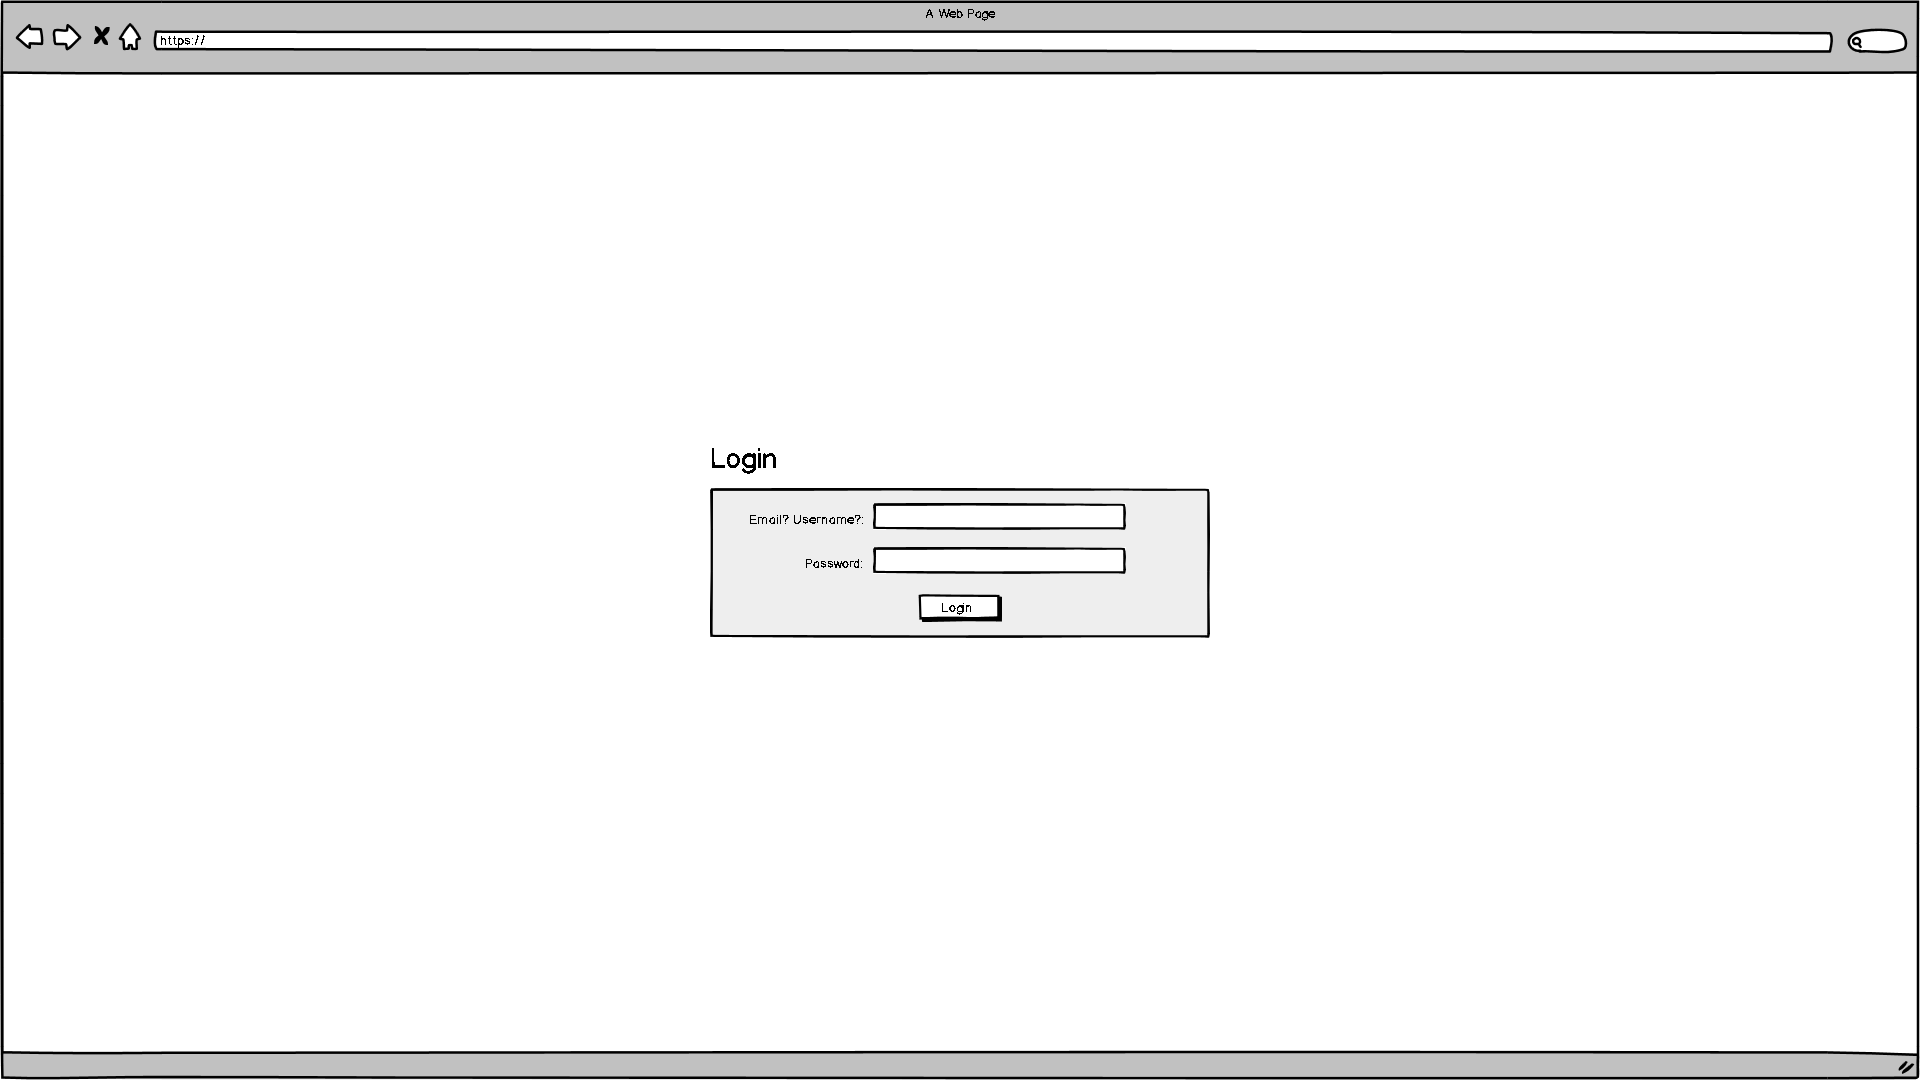
\includegraphics[width=\textwidth]{Images/01MWL.png}
	\caption{The Login Windows shown as the page is first loaded}
	\label{fig:loginWindow}
\end{figure}


\begin{figure}[ht]
	\centering
	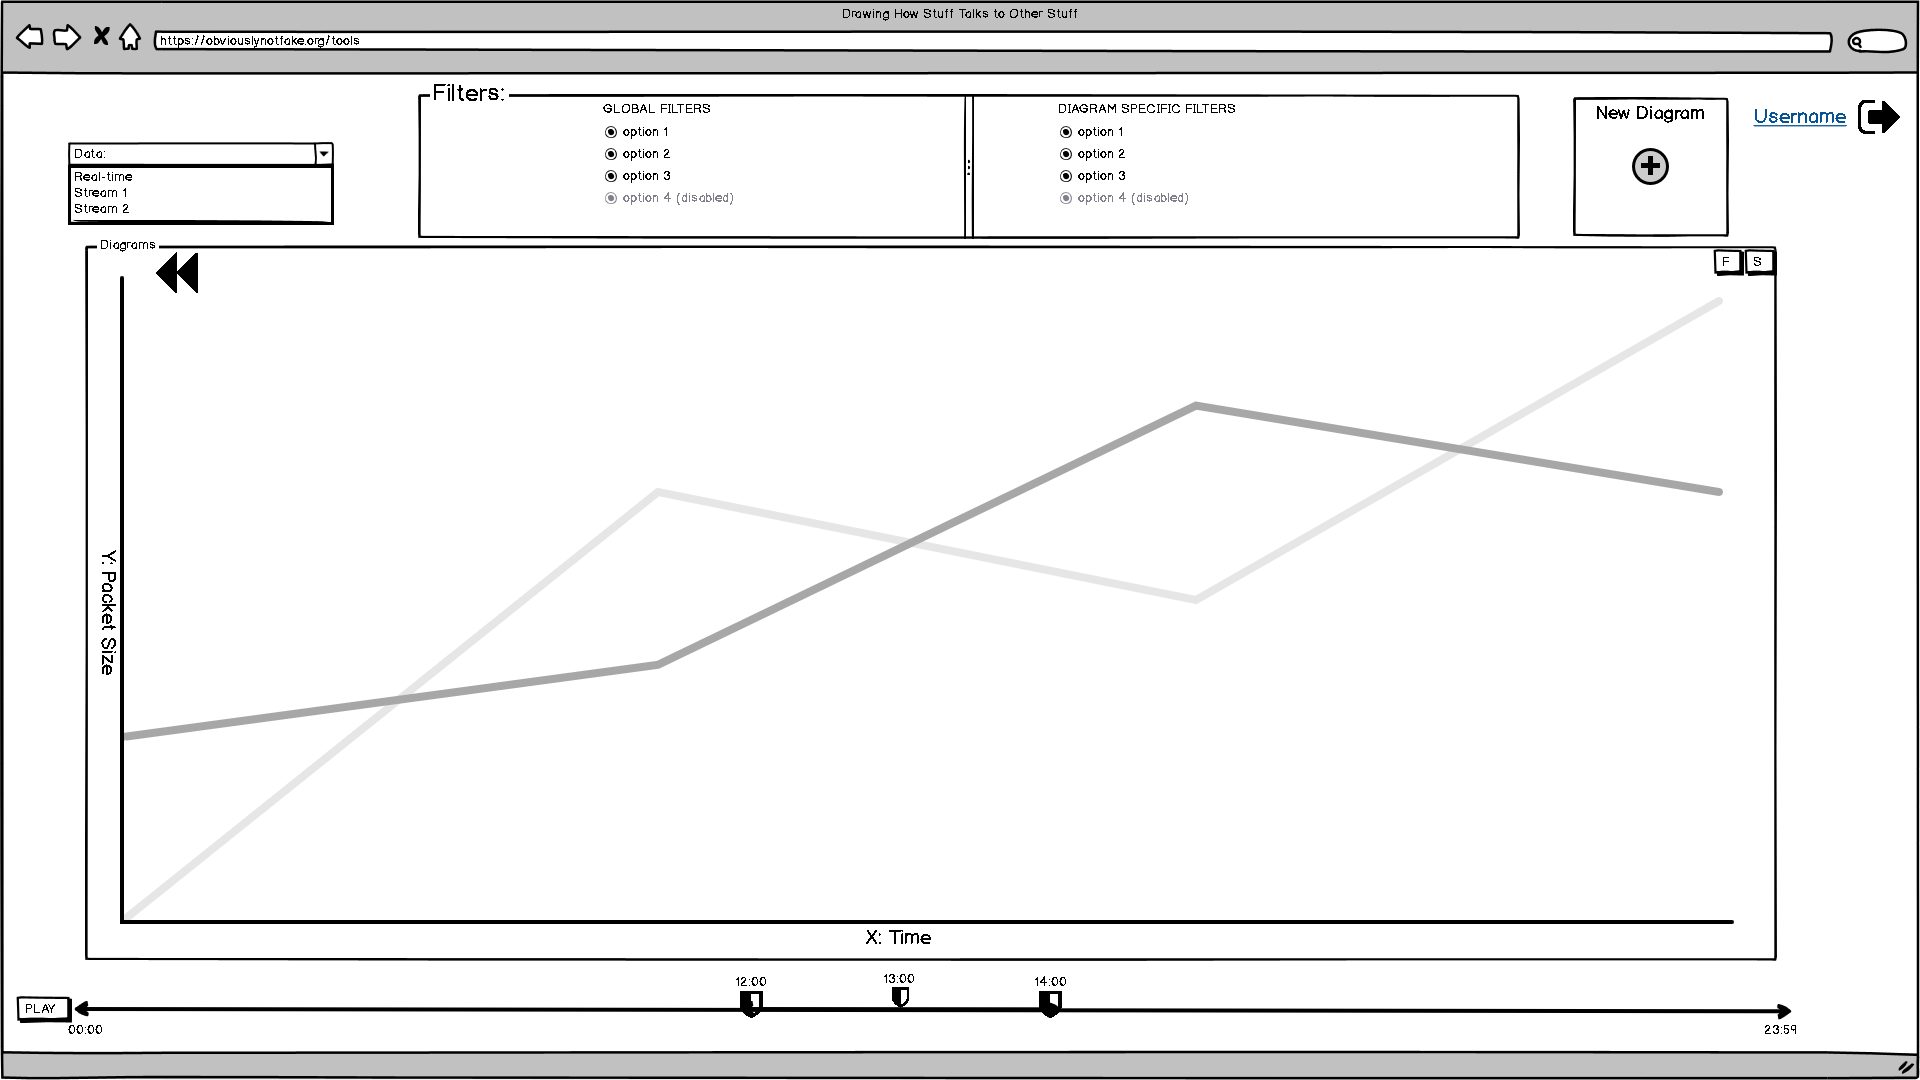
\includegraphics[width=\textwidth]{Images/02MW.png}
	\caption{The Main window the user sees once he logs in}
	\label{fig:mainWindow0}
\end{figure}
\vfill
\clearpage

To discuss in depth this interface it has been divided into subsections labeled in \autoref{fig:mainWindow5}, these are:
\\
\begin{enumerate}
	\item The Data stream drop down menu allows the user to select which stream he is currently listening to. This dropdown menu shows the selected diagram's selected data stream and by default is set to real-time.
	\item Here the user can set filters affecting all diagrams, namely limiting which layers and protocols are currently being shown. To add a new filter a user would click on the add filter button, select which part of the data stream is to be used in the filter, any optional comparators, and set a parameter in the text-box.
	\item This button opens the diagram filter list, this list contains filters specific to each diagram.
	\item By clicking this button the user can create a new diagram shown in number 5. The creation workflow is shown in \autoref{fig:mainWindow1} to \autoref{fig:mainWindow5}.
	\item Here is the currently logged in user, by clicking the button to the right of his name the user can log out.
	\item This is the \gls{diagram container}, inside are all diagrams the user has created with all the set constraints. At most 4 diagrams are shown in the container, and more can be made visible via the slider on the right of the container.
	\item This is a diagram.
	\item By hovering with the mouse over a data point a tooltip is shown with all data associated with this data point.
	\item These buttons control whether a diagram is fullscreen and the diagram settings. By clicking the button labeled F the diagram grows to take on all available space in the container, like shown in \autoref{fig:mainWindow0}.
	      \\
	      Clicking on the button labeled "S" replaces the diagram with the Settings for this diagram like shown in \autoref{fig:mainWindow1}
	\item The play button starts and stops auto scroll along the selected time frame
	\item This timeline shows on the left and right bottom labels the beginning and end of all data streams. The labels on top show the currently selected time window and are movable to increasea nd decrease the time window. The middle shield icon shows the current time while being played, and is also movable to scroll by data manually.

\end{enumerate}


\vfill

\begin{figure}[ht]
	\centering
	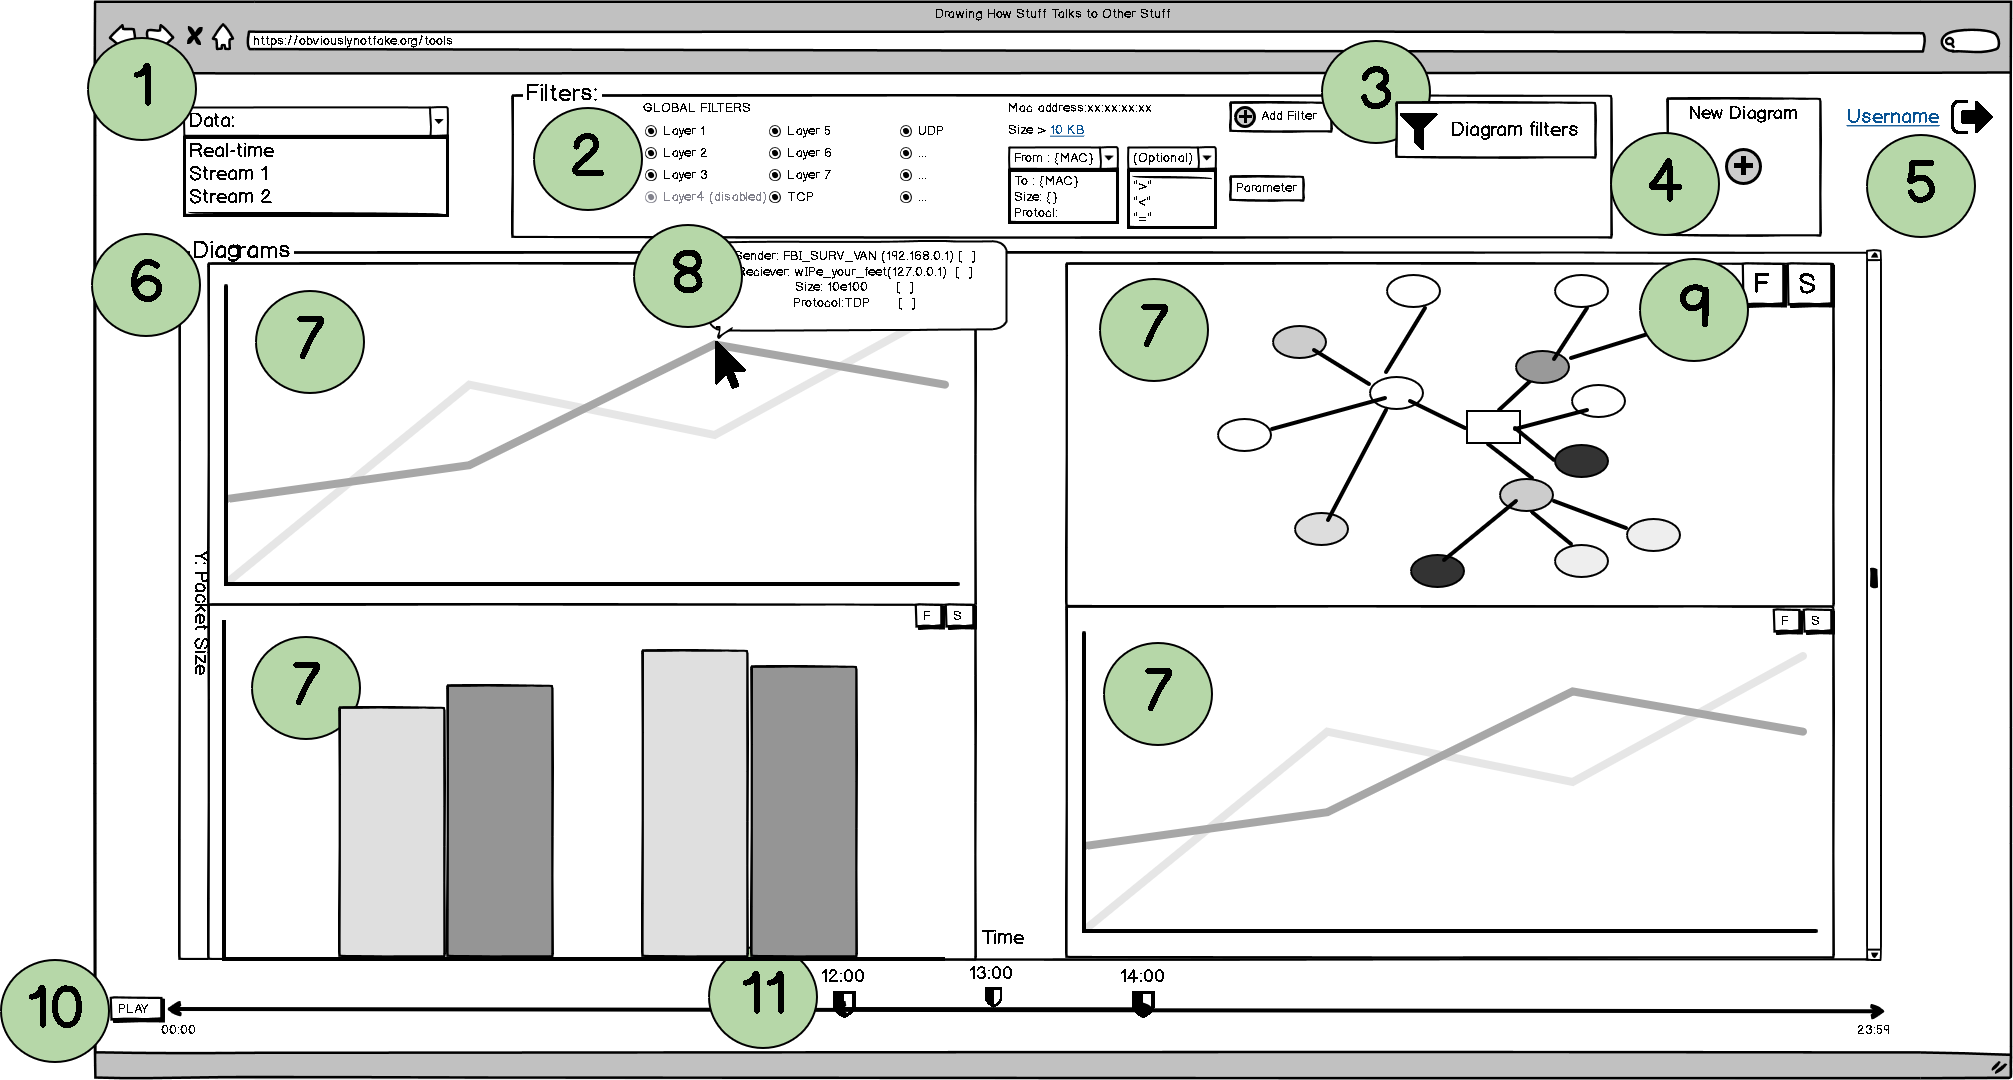
\includegraphics[width=\textwidth]{Images/07MW.png}
	\caption{The GUI divided into relevant sections}
	\label{fig:mainWindow5}
\end{figure}

\vfill
\clearpage

Next we'll take a look at the workflow a user will go through when opening a new diagram.
\\
As referenced above \autoref{fig:mainWindow0} is what the user first sees. When he wants to create a new diagram, by clicking the button labeled new diagram, the Main window is split (shown in \autoref{fig:mainWindow1}) and the new diagram settings are shwon where the new diagram will be.
\\
The user sets here the settings for the new diagram, these are:
\\
\begin{itemize}
	\item{Which data stream it draws its data from}
	\item{Which data is pulled to be represented as the x and y axis}
	\item{Any filters the user wants to apply at the start}
\end{itemize}

Afterwards, the screen looks like \autoref{fig:mainWindow2}, the \gls{diagram container} split in half. By going through this process two more times the diagram container fills up, containing four diagrams total (shown in \autoref{fig:mainWindow3}); at this point the diagrams have their minimum size.
\\
Any diagrams created afterwards are spawned underneath the existing ones and the user can scroll up and down to view all of them (shown in \autoref{fig:mainWindow4}) (TBD)



\vfill

\begin{figure}[h]
	\centering
	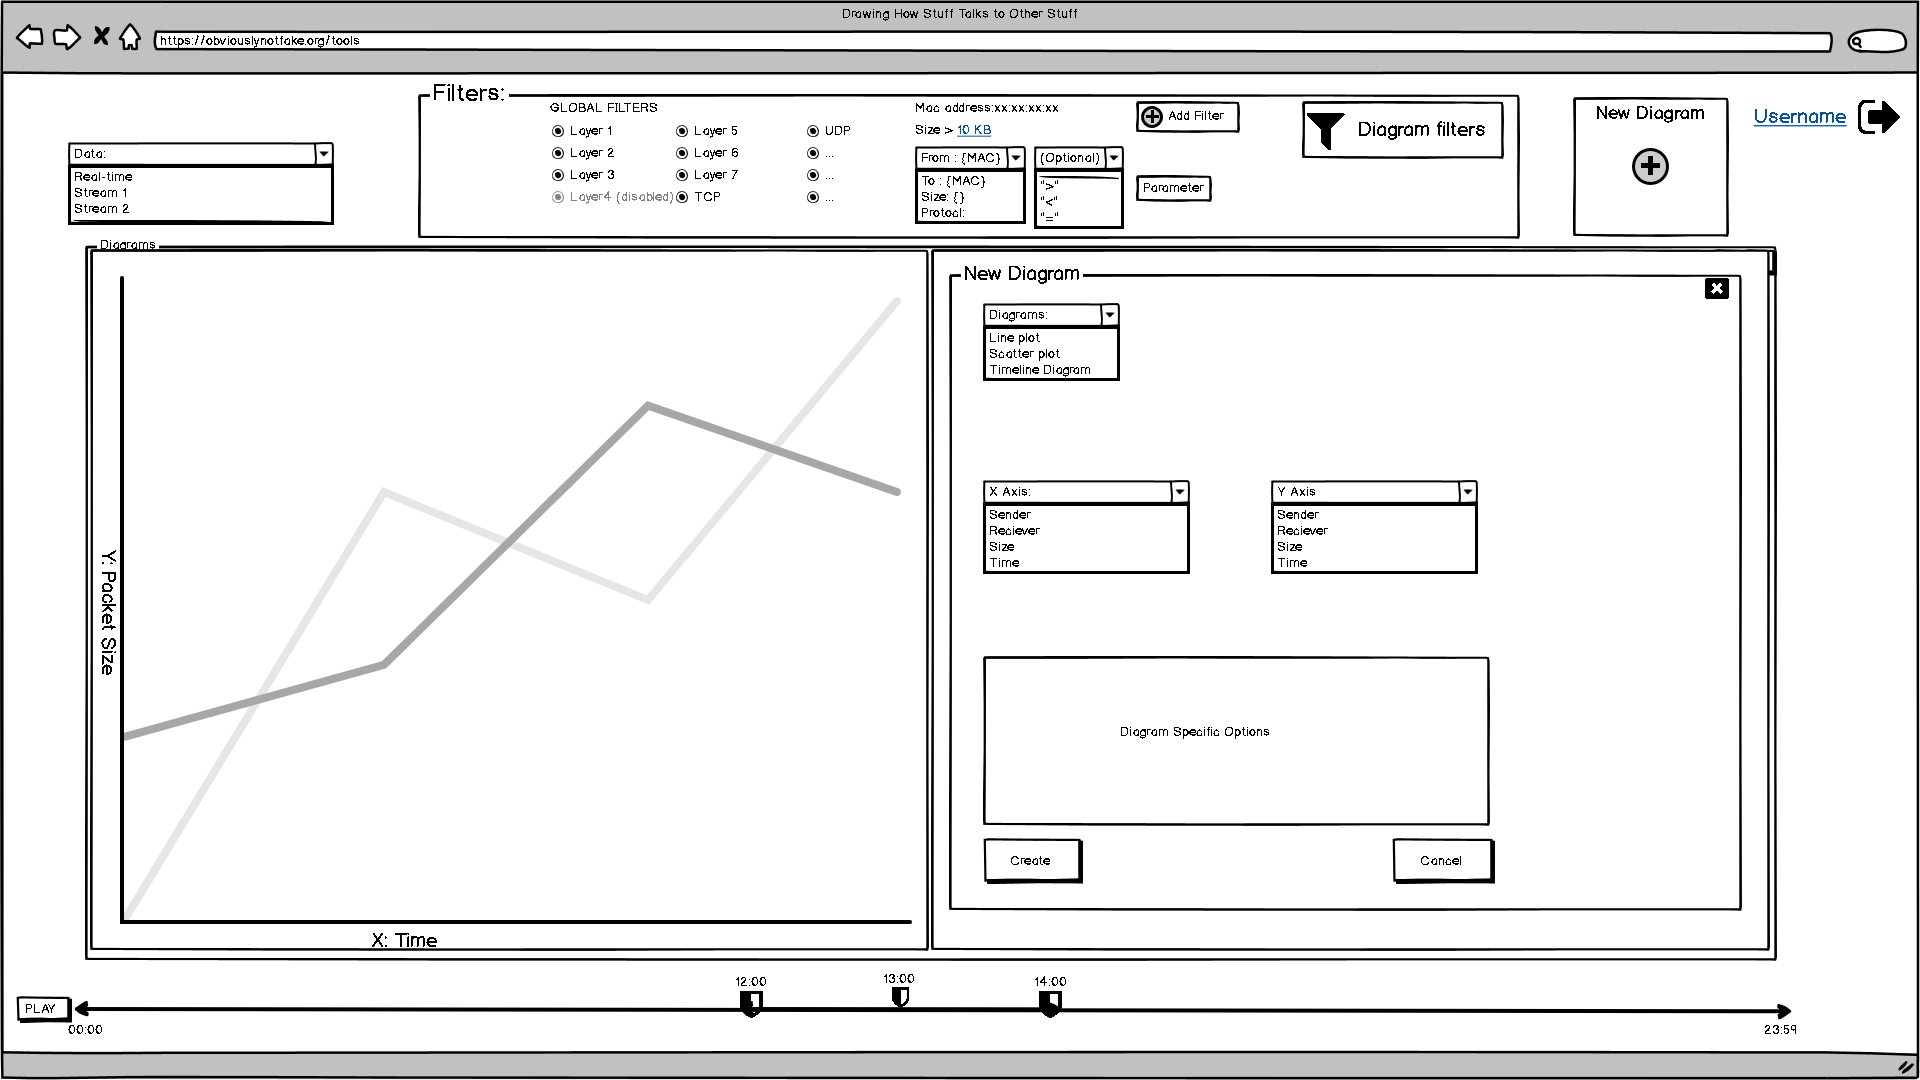
\includegraphics[width=\textwidth]{Images/03MW.png}
	\caption{Main window split in two after user has clicked on the "New diagram" button. New diagram options are set up on the right.}
	\label{fig:mainWindow1}
\end{figure}


\vfill

\begin{figure}[h]
	\centering
	\label{fig:mainWindow2}
	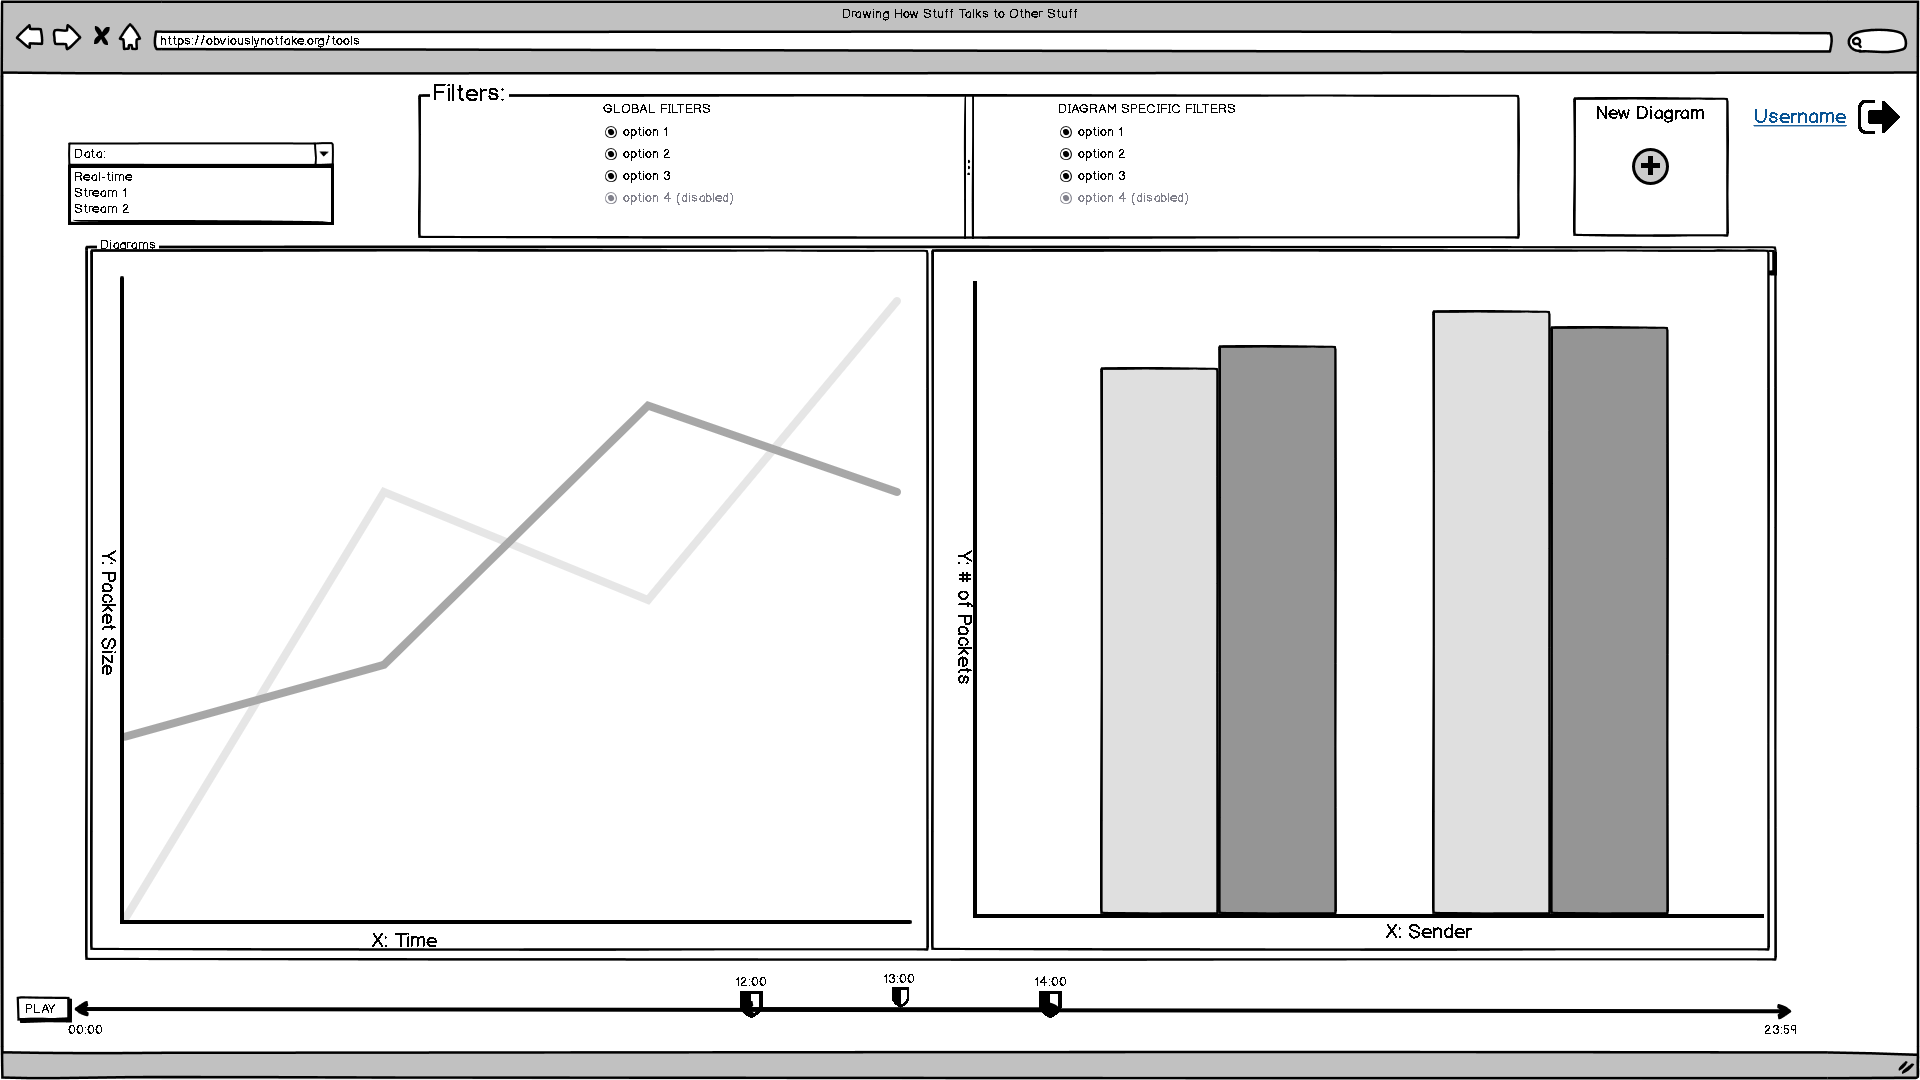
\includegraphics[width=\textwidth]{Images/04MW.png}
	\caption{Main Window with two diagrams side by side.}
	\label{fig:mainWindow2}
\end{figure}



\begin{figure}[h]
	\centering
	\label{fig:mainWindow3}
	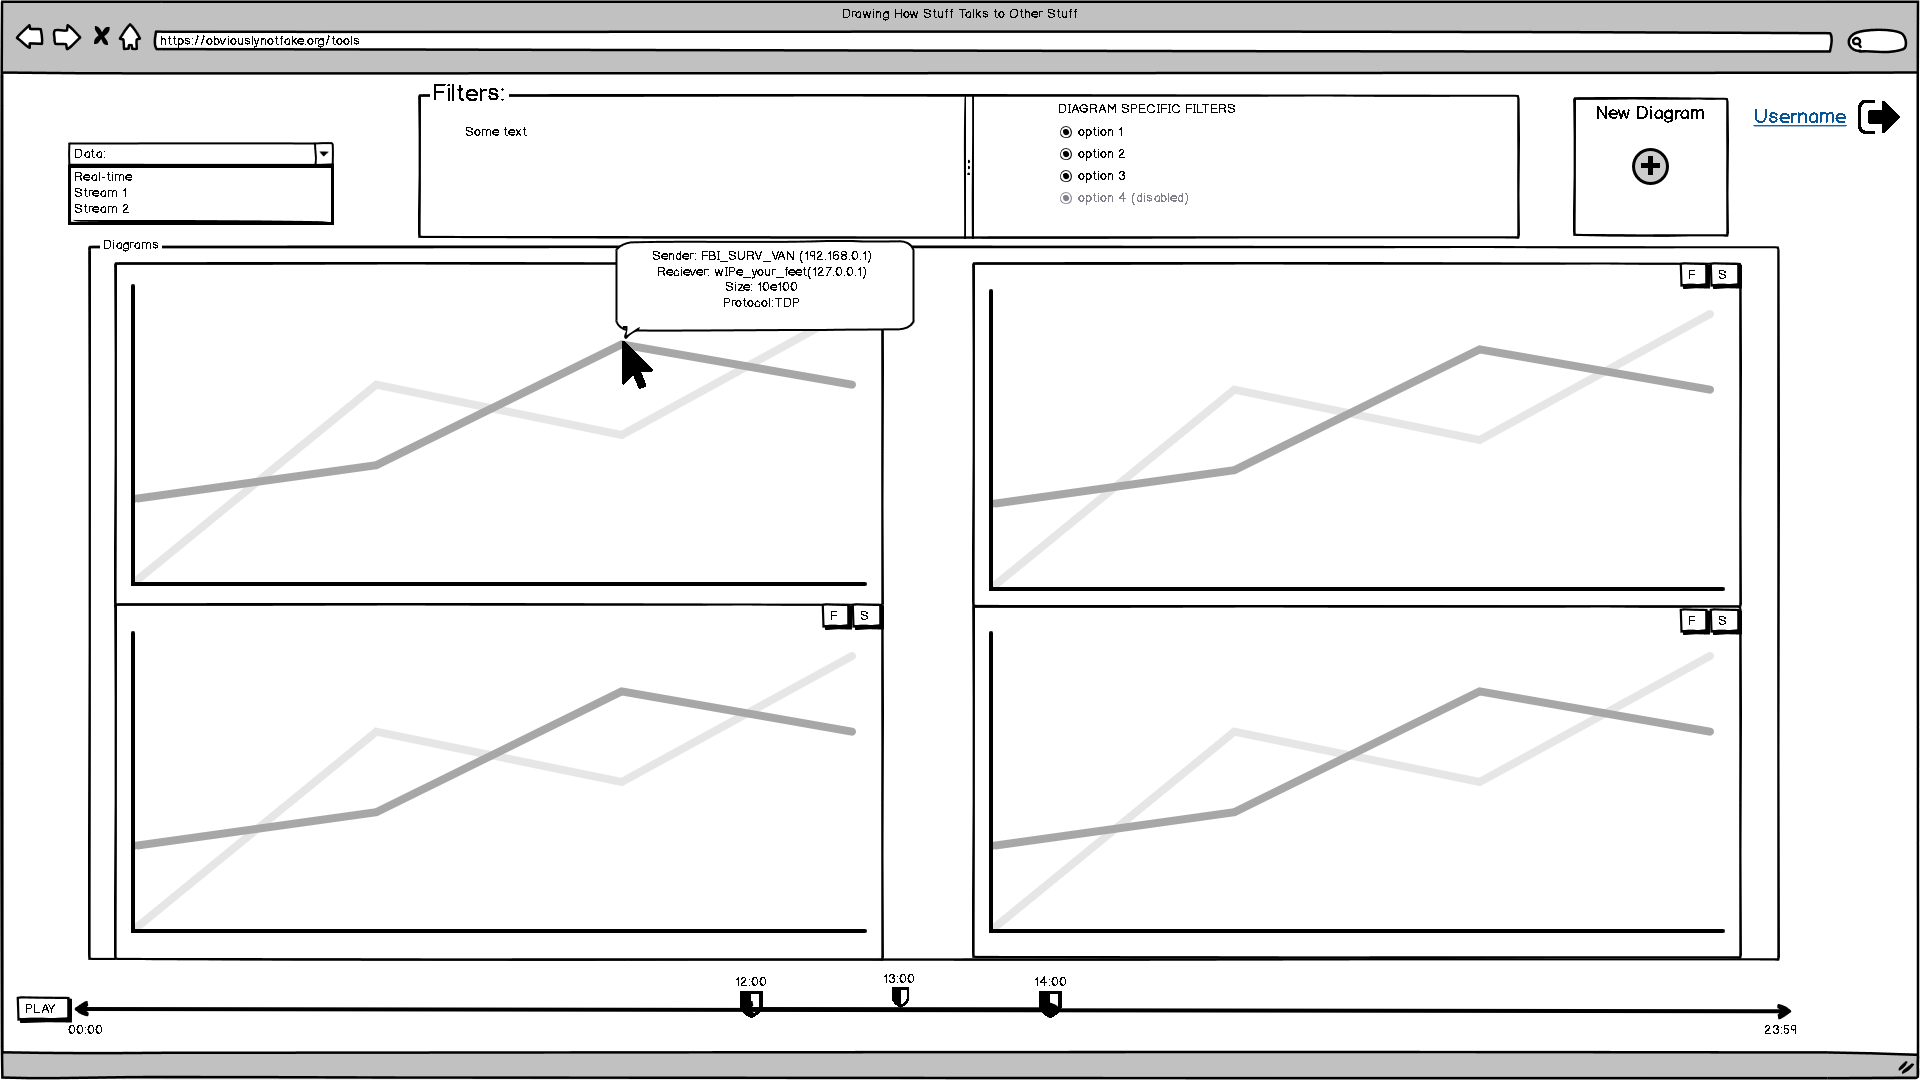
\includegraphics[width=\textwidth]{Images/05MW.png}
	\caption{Main window with four diagrams open}
	\label{fig:mainWindow3}
\end{figure}

\begin{figure}[h]
	\centering
	\label{fig:mainWindow4}
	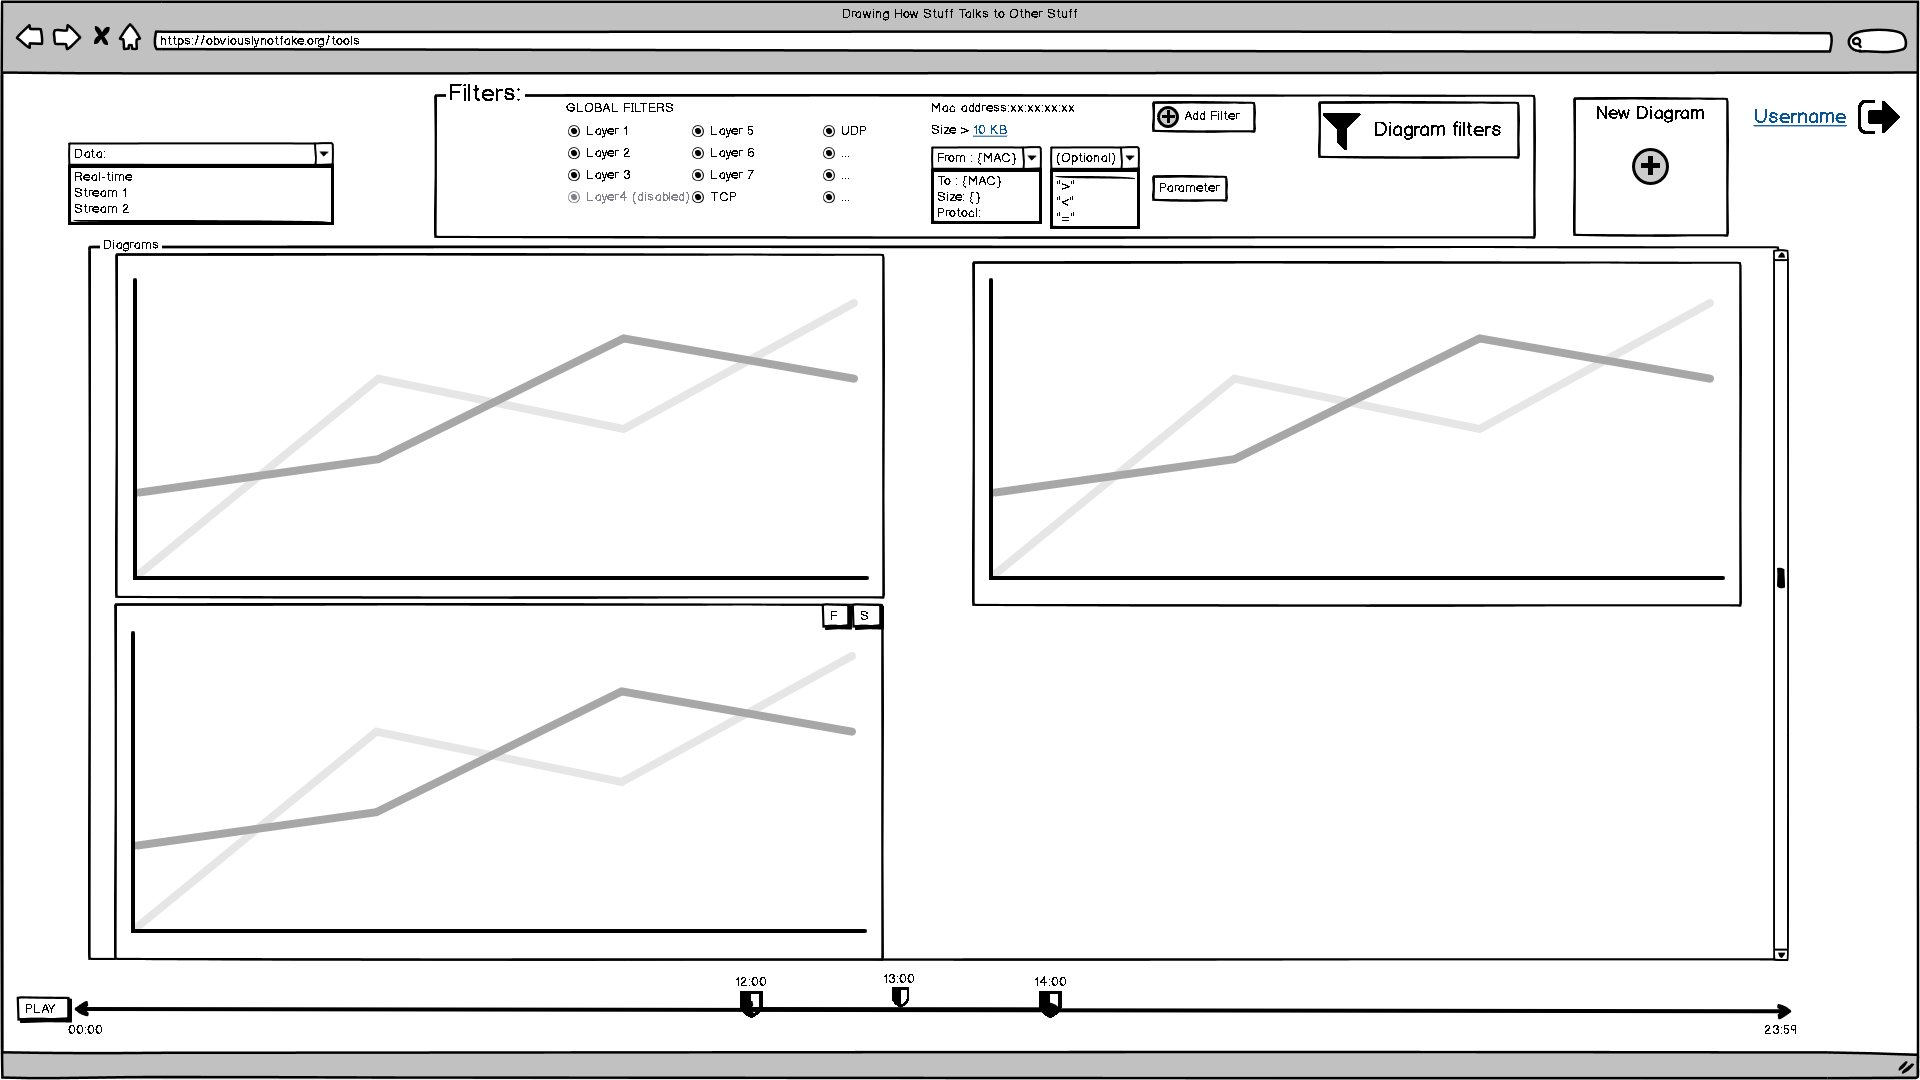
\includegraphics[width=\textwidth]{Images/06MW.png}
	\caption{Main window with more than four diagrams open, more diagrams can be shown using the scroll bar}
	\label{fig:mainWindow4}
\end{figure}

Another activity the user will use frequently is the filtering system.
\\
In the previous section we took a look at the Main window and its different sections, there we described that filters that apply to every diagram are shown at all times shown as item 2. But what about when you want to create a filter that only affects one diagram?
\\
For that, the user would click on the Diagram filter (see previous section), an overlay would cover the whole window and a new set of containers, similar to the global filter, would appear. As seen on \autoref{fig:mainWindow6}
\\
On the top we see the global filter list, below it we see the filter list corresponding to the first diagram (diagram numbering is done left to right and top to bottom).
\\
In order to set a new filter that applies to only one diagram the user would open this screen, search for the corresponding diagram number and click on the "add filter button" at which point the button get's moved down to make space for a drop down menu containing all types of data from a data stream. The user selects one, and depending on which one, if appropriate, another drop down menu appears, with contextual relational symbols (i.e. less than (<), equals, etc.) and next to it a text box where the user can input the matching string to which to filter.


\begin{figure}[h]
	\centering
	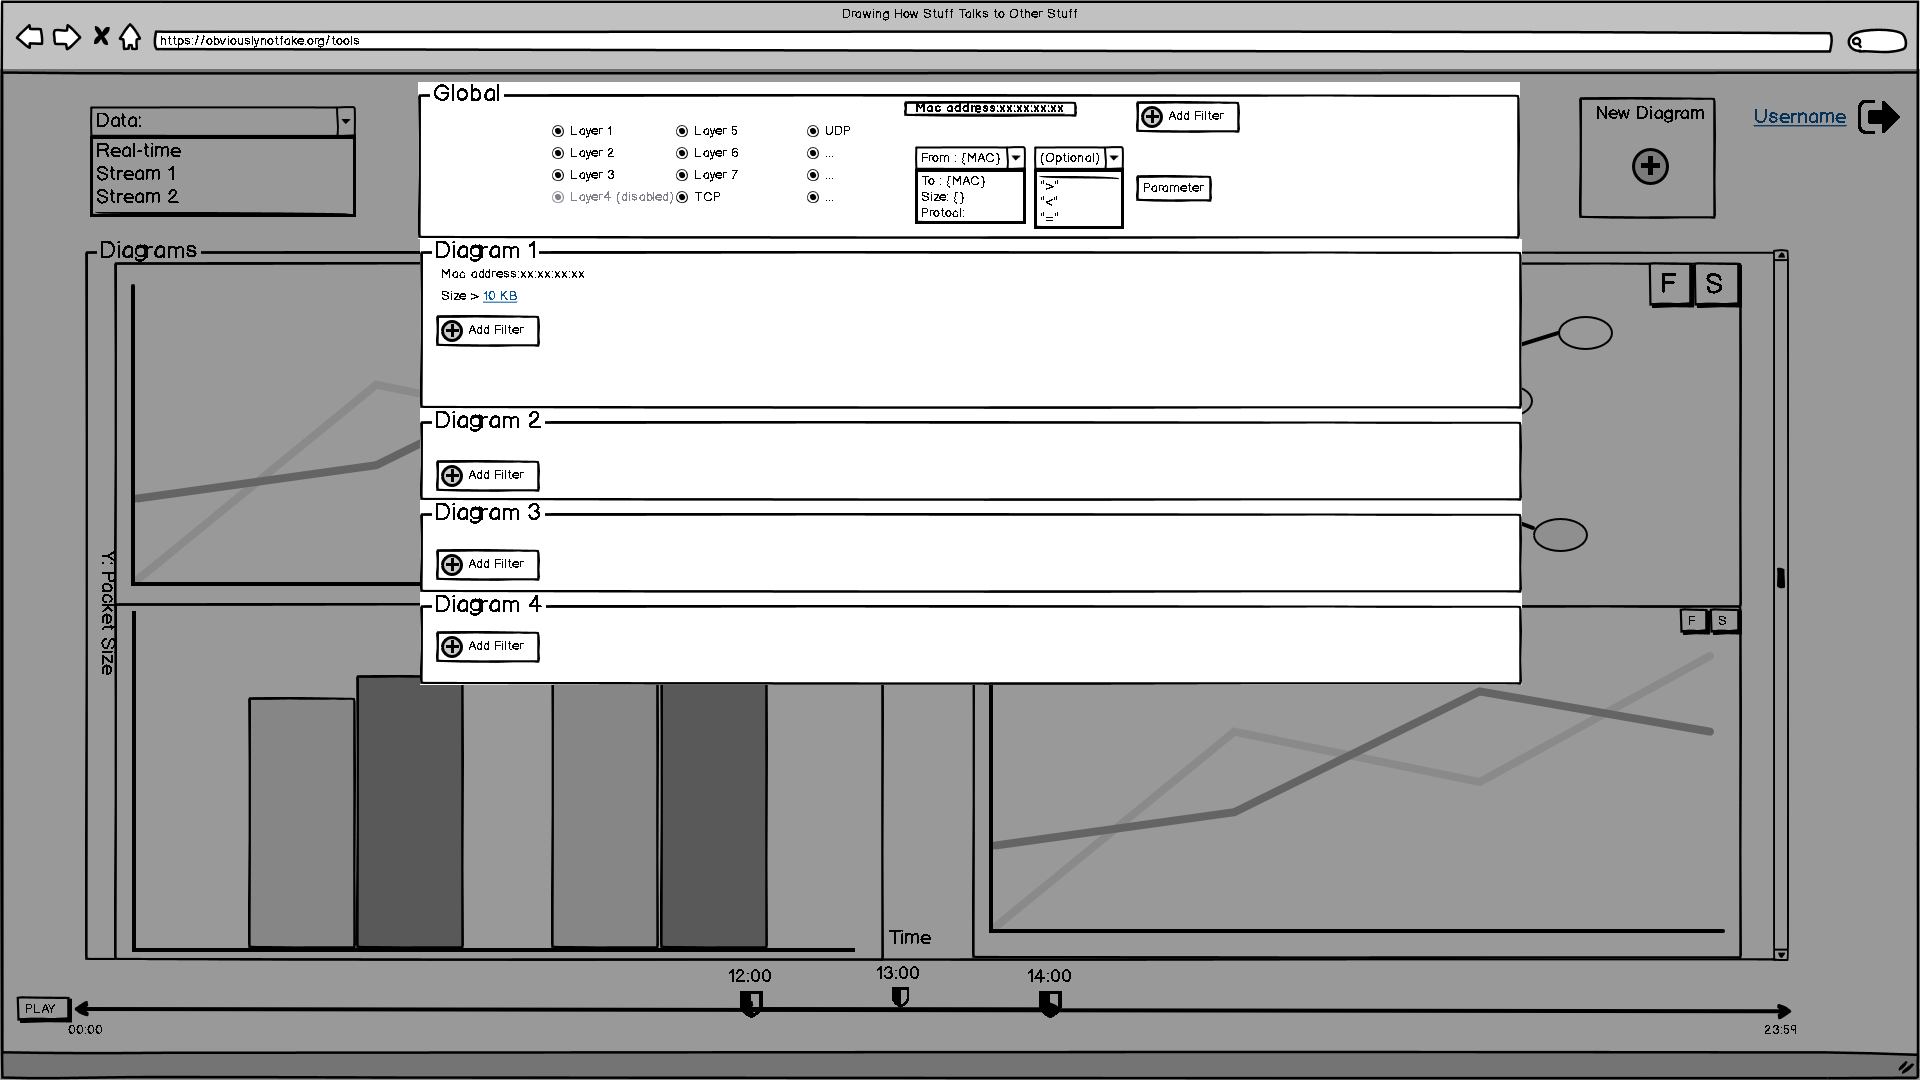
\includegraphics[width=\textwidth]{Images/09MW.png}
	\caption{Main window with more than four diagrams open, more diagrams can be shown using the scroll bar}
	\label{fig:mainWindow6}
\end{figure}

%added this to show all images on GUI section
\clearpage

\subsubsection{Diagram types}
%scatter plot
%https://commons.wikimedia.org/wiki/File:Scatter_diagram_for_quality_characteristic_XXX.svg

Next we'll discuss the four basic diagram types that comprise the minimum scope of this project and their possible use cases.
These are:

Line chart: to easily compare ,linearly, two variables from a data stream.(\autoref{fig:linechart})
\\
Network Diagram: provides a simple way to visualize the network topology. This diagram also gives the user the ability to inspect the nodes of the network and select data from a data point to be used as a filter in other diagrams (refer to last section for usage example).
(\autoref{fig:netdiaram})
\\
Raster spike diagram: this is useful to show the transmission window of each packet and it's corresponding partner.(\autoref{fig:rasterplot})
\\
Scatter plot: a way to visualize up to 4 dimensions of the data stream.(\autoref{fig:scatterplot})
\\
These are examples and since the user has the ability to chose what part of the data stream is used for each axis it does not convey the full ability of these diagrams, that is left to the end user.


\begin{figure*}[!h]
	\centering
	\begin{subfigure}[h]{0.475\textwidth}
		\centering
		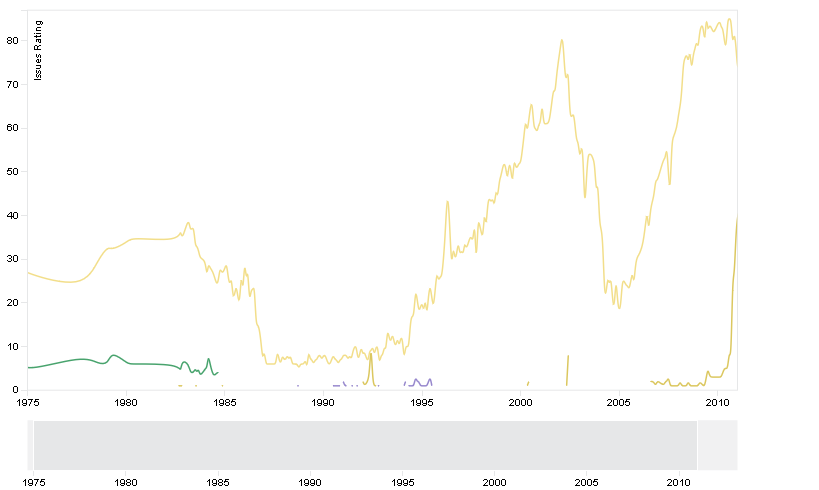
\includegraphics[width=\textwidth]{Images/line_chart.png}
		\caption[Line Chart]%
		{{\small Line Chart}}
		\label{fig:Diagram types}
	\end{subfigure}
	\hfill
	\begin{subfigure}[h]{0.475\textwidth}
		\centering
		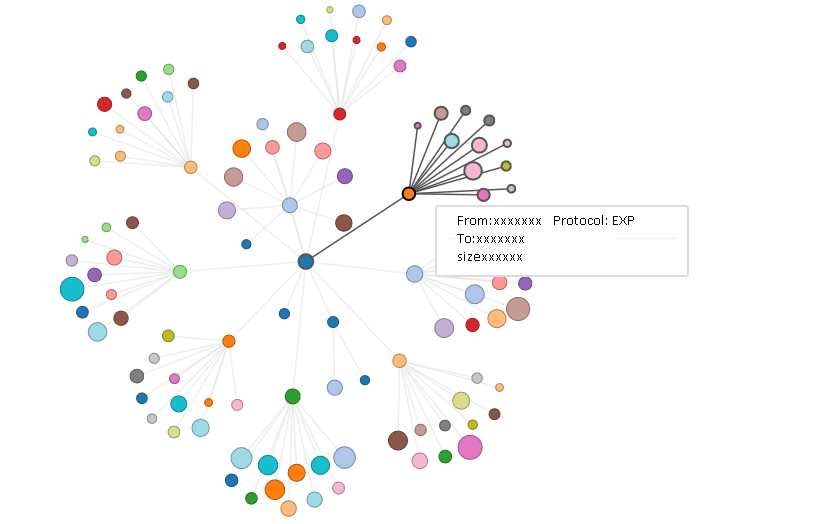
\includegraphics[width=\textwidth]{Images/net_diag.png}
		\caption[]%
		{{\small Net diagram}}
		\label{fig:Diagram types}
	\end{subfigure}
	\vskip\baselineskip
	\begin{subfigure}[h]{0.475\textwidth}
		\centering
		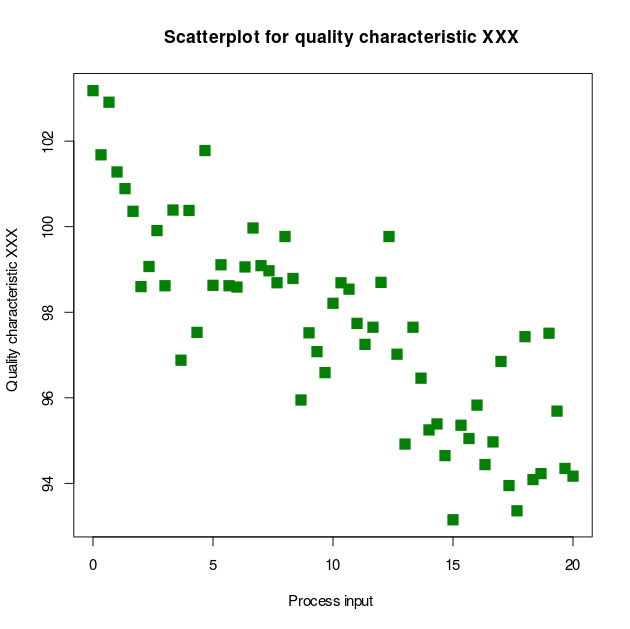
\includegraphics[width=\textwidth]{Images/Scatter_diagram.png}
		\caption[]%
		{{\small Scatterdiagram}}
		\label{fig:Diagram types}
	\end{subfigure}
	\quad
	\begin{subfigure}[h]{0.475\textwidth}
		\centering
		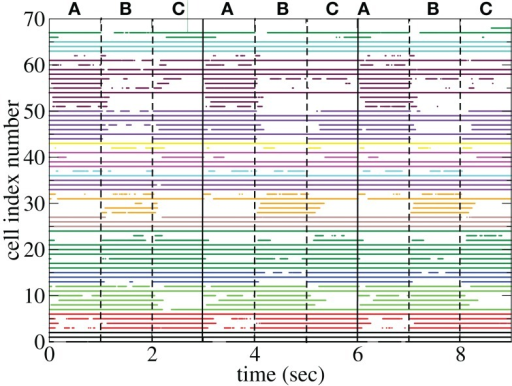
\includegraphics[width=\textwidth]{Images/spike_raster_plot.png}
		\caption[]%
		{{\small Spike raster plot}}
		\label{fig:mean and std of net44}
	\end{subfigure}
	\caption[ Diagram types ]
	{\small Diagram types}
	\label{fig:Diagram types}
\end{figure*}
\vfill

\subsection{Scenarios}

\begin{description}
	\item[S100:] An operator wants to check manually/visually whether network nodes appeared or disappeared over the last day
	      \begin{itemize}
		      \item{the operator opens the web page}
		      \item{the operator selects the database as \gls{data source}}
		      \item{the operator selects a time-line-based \gls{diagram type}}
		      \item{the operator selects node addresses as the data to be displayed}
		      \item{the operator moves to or selects the last 24 hours as the range of data to display}
		      \item{the operator closes the web page}
	      \end{itemize}



	\item[S200:] A security analyst wants to look at the current flow rates between network nodes to see whether they change / there are trends
	      \begin{itemize}
		      \item{the analyst opens the web page}
		      \item{the analyst selects a source of live data}
		      \item{the analyst selects an appropriate visualization type}
		      \item{the analyst selects node addresses as the independent variable}
		      \item{the analyst selects flow rates as the data to be displayed}
	      \end{itemize}



	\item[S300:] A security analyst wants to examine a specific point of data
	      \\
	      Precondition: the analyst has already selected the relevant dataset and visualization type
	      \begin{itemize}
		      \item{the analyst selects a data point}
		      \item{the GUI displays a small pop-up window with all the data of this data point}
		      \item{the analyst right-clicks one of the attibutes in the pop-up window and selects "Display all matching types"}
		      \item{the GUI marks all data points that have the same value in this attribute}
	      \end{itemize}



	\item[S400:] The user wants to look at alarms/notifications (TBD)
	      \begin{itemize}
		      \item{the user opens the web page}
		      \item{the user selects the database as data source}
		      \item{the user selects the data stream from the relevant dissector}
		      \item{the GUI diplays the notifications along a timeline, according oder of occurance}
		      \item{the user right-clicks on the x-axis and selects "use record number"}
		      \item{the GUI diplays the notifications along a timeline adjacently}
	      \end{itemize}



	\item[S500:] The user wants to look at normal data together with alarms/notifications
	      \\
	      Precondition: Scenario S100 apart from closing the web page
	      \begin{itemize}
		      \item{the user selects menu "data", entry "sources"}
		      \item{the GUI displays a list of all known data sources with a checkbox in front of each}
		      \item{the user selects the checkboxes for the data sources they want to examine}
		      \item{the GUI displays data from all these data sources within the currently active visualization}
	      \end{itemize}


\end{description}

\subsection{Use cases}
\begin{figure}[h]
	\centering
	\includegraphics[width=\textwidth]{Images/case_login.png}
	\caption{User Login.}
\end{figure}

\begin{description}
	\item[Use Case UC1: Login]
	      \hfill
	      \begin{description}
		      \item[Scope:] ADIN Inspector and hub
		      \item[Level:] user goal
		      \item[Stakeholders and Interests:]
		            \hfill
		            \begin{itemize}
			            \item{User: Wants to login quickly and easily}
			            \item{System administrator: Wants to ensure that only authorized persons access the system. Wants few user support requests.}
			            \item{Manager: Wants protection of data. Wants no obstacle to the user's work.}
		            \end{itemize}
		      \item[Preconditions:] An account for the user has been created.
		      \item[Postconditions:] User is loged in.
		      \item[Main Success Scenario:]
		            \hfill
		            \begin{enumerate}
			            \item{Customer opens the ADIN website in the browser}
			            \item{Customer enters his/her username and password}
			            \item{The ADIN system checks the entered password and loads the access permissions for the user.}
			            \item{The sytem presents the ADIN main screen.}
			            \item{User begins to use the ADIN Inspector.}
		            \end{enumerate}

		      \item[Extensions:]
		            \hfill
		            \begin{itemize}
			            \item[]*a. At any time, the network connection to the server fails or the server crashes:
			                  \begin{enumerate}
				                  \item{the user reloads the web site which takes him/her to the ADIN login screen}
			                  \end{enumerate}

			            \item[]3a. Wrong username or password:
			                  \begin{enumerate}
				                  \item{System produces an error message and stays on the login screen.}
			                  \end{enumerate}

		            \end{itemize}
	      \end{description}

	      \begin{figure}[h]
		      \centering
		      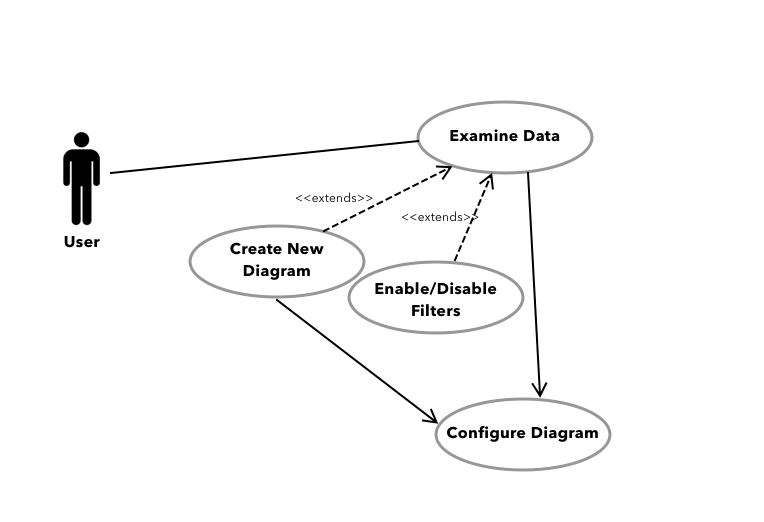
\includegraphics[width=\textwidth]{Images/case_examine_data.png}
		      \caption{Examine Data.}
	      \end{figure}
\end{description}


\subsubsection{Interactivity}

Visual analytics methods combine interactive visualisations with automated analysis
techniques. This allows the user to decide e.g. which part
of the data he or she wants to explore in more detail.

A basic principle for visual data exploration was introduced by Shneiderman (1997) by what he called the “The Visual Information Seeking Mantra:

Overview first, zoom and filter, then details-ondemand”.
This lets the data analyst define to a certain level what he or she wants
to see and visualise.

Similar to this, Bertin (1983) specified three “levels of reading,”:
The elementary level (allowing the analyst to look at the information about a
single data record), the intermediate level (showing summarised information about a group of data records), and the global level (providing an overview of all data elements).

\subsection{Object Modelling}

The following diagram shows a high-level view of the components of the ADIN-Inspector. The PSE group will develop the visualization component that runs in the web browser and a server side component called hub. The hub interfaces with the data sources and also implements the access control.

\begin{center}
	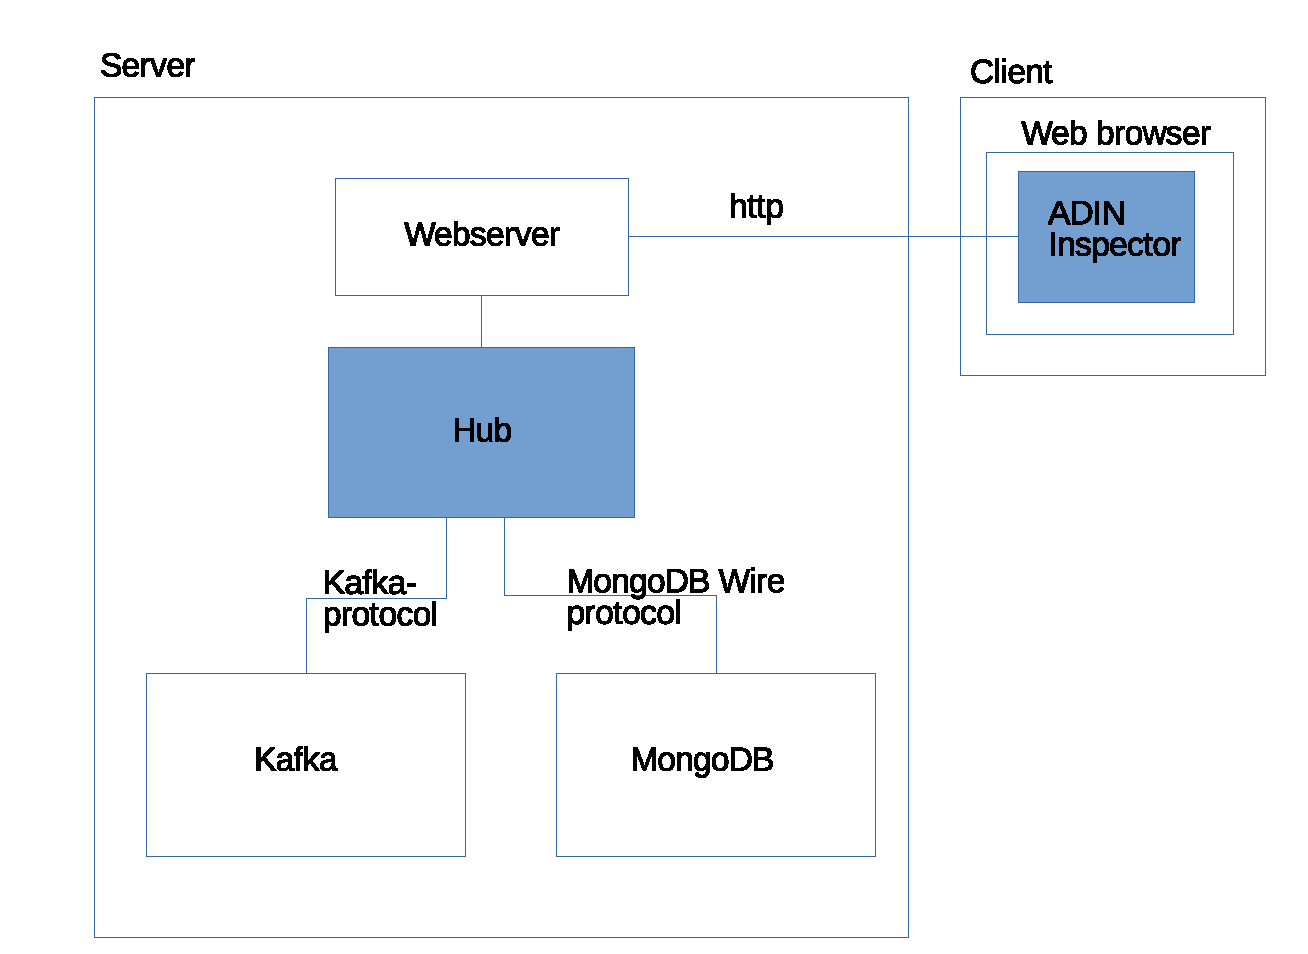
\includegraphics[scale=0.8]{Images/adin-sys1d.eps}
	\captionof{figure}{General system layout. Components to be developed by the PSE group are marked blue.}
	\label{fig:adinsys1c}
\end{center}


\subsection{Dynamic Modelling}

\autoref{fig:adin-login-seq} shows the actions of the Hub component during login.

\begin{center}
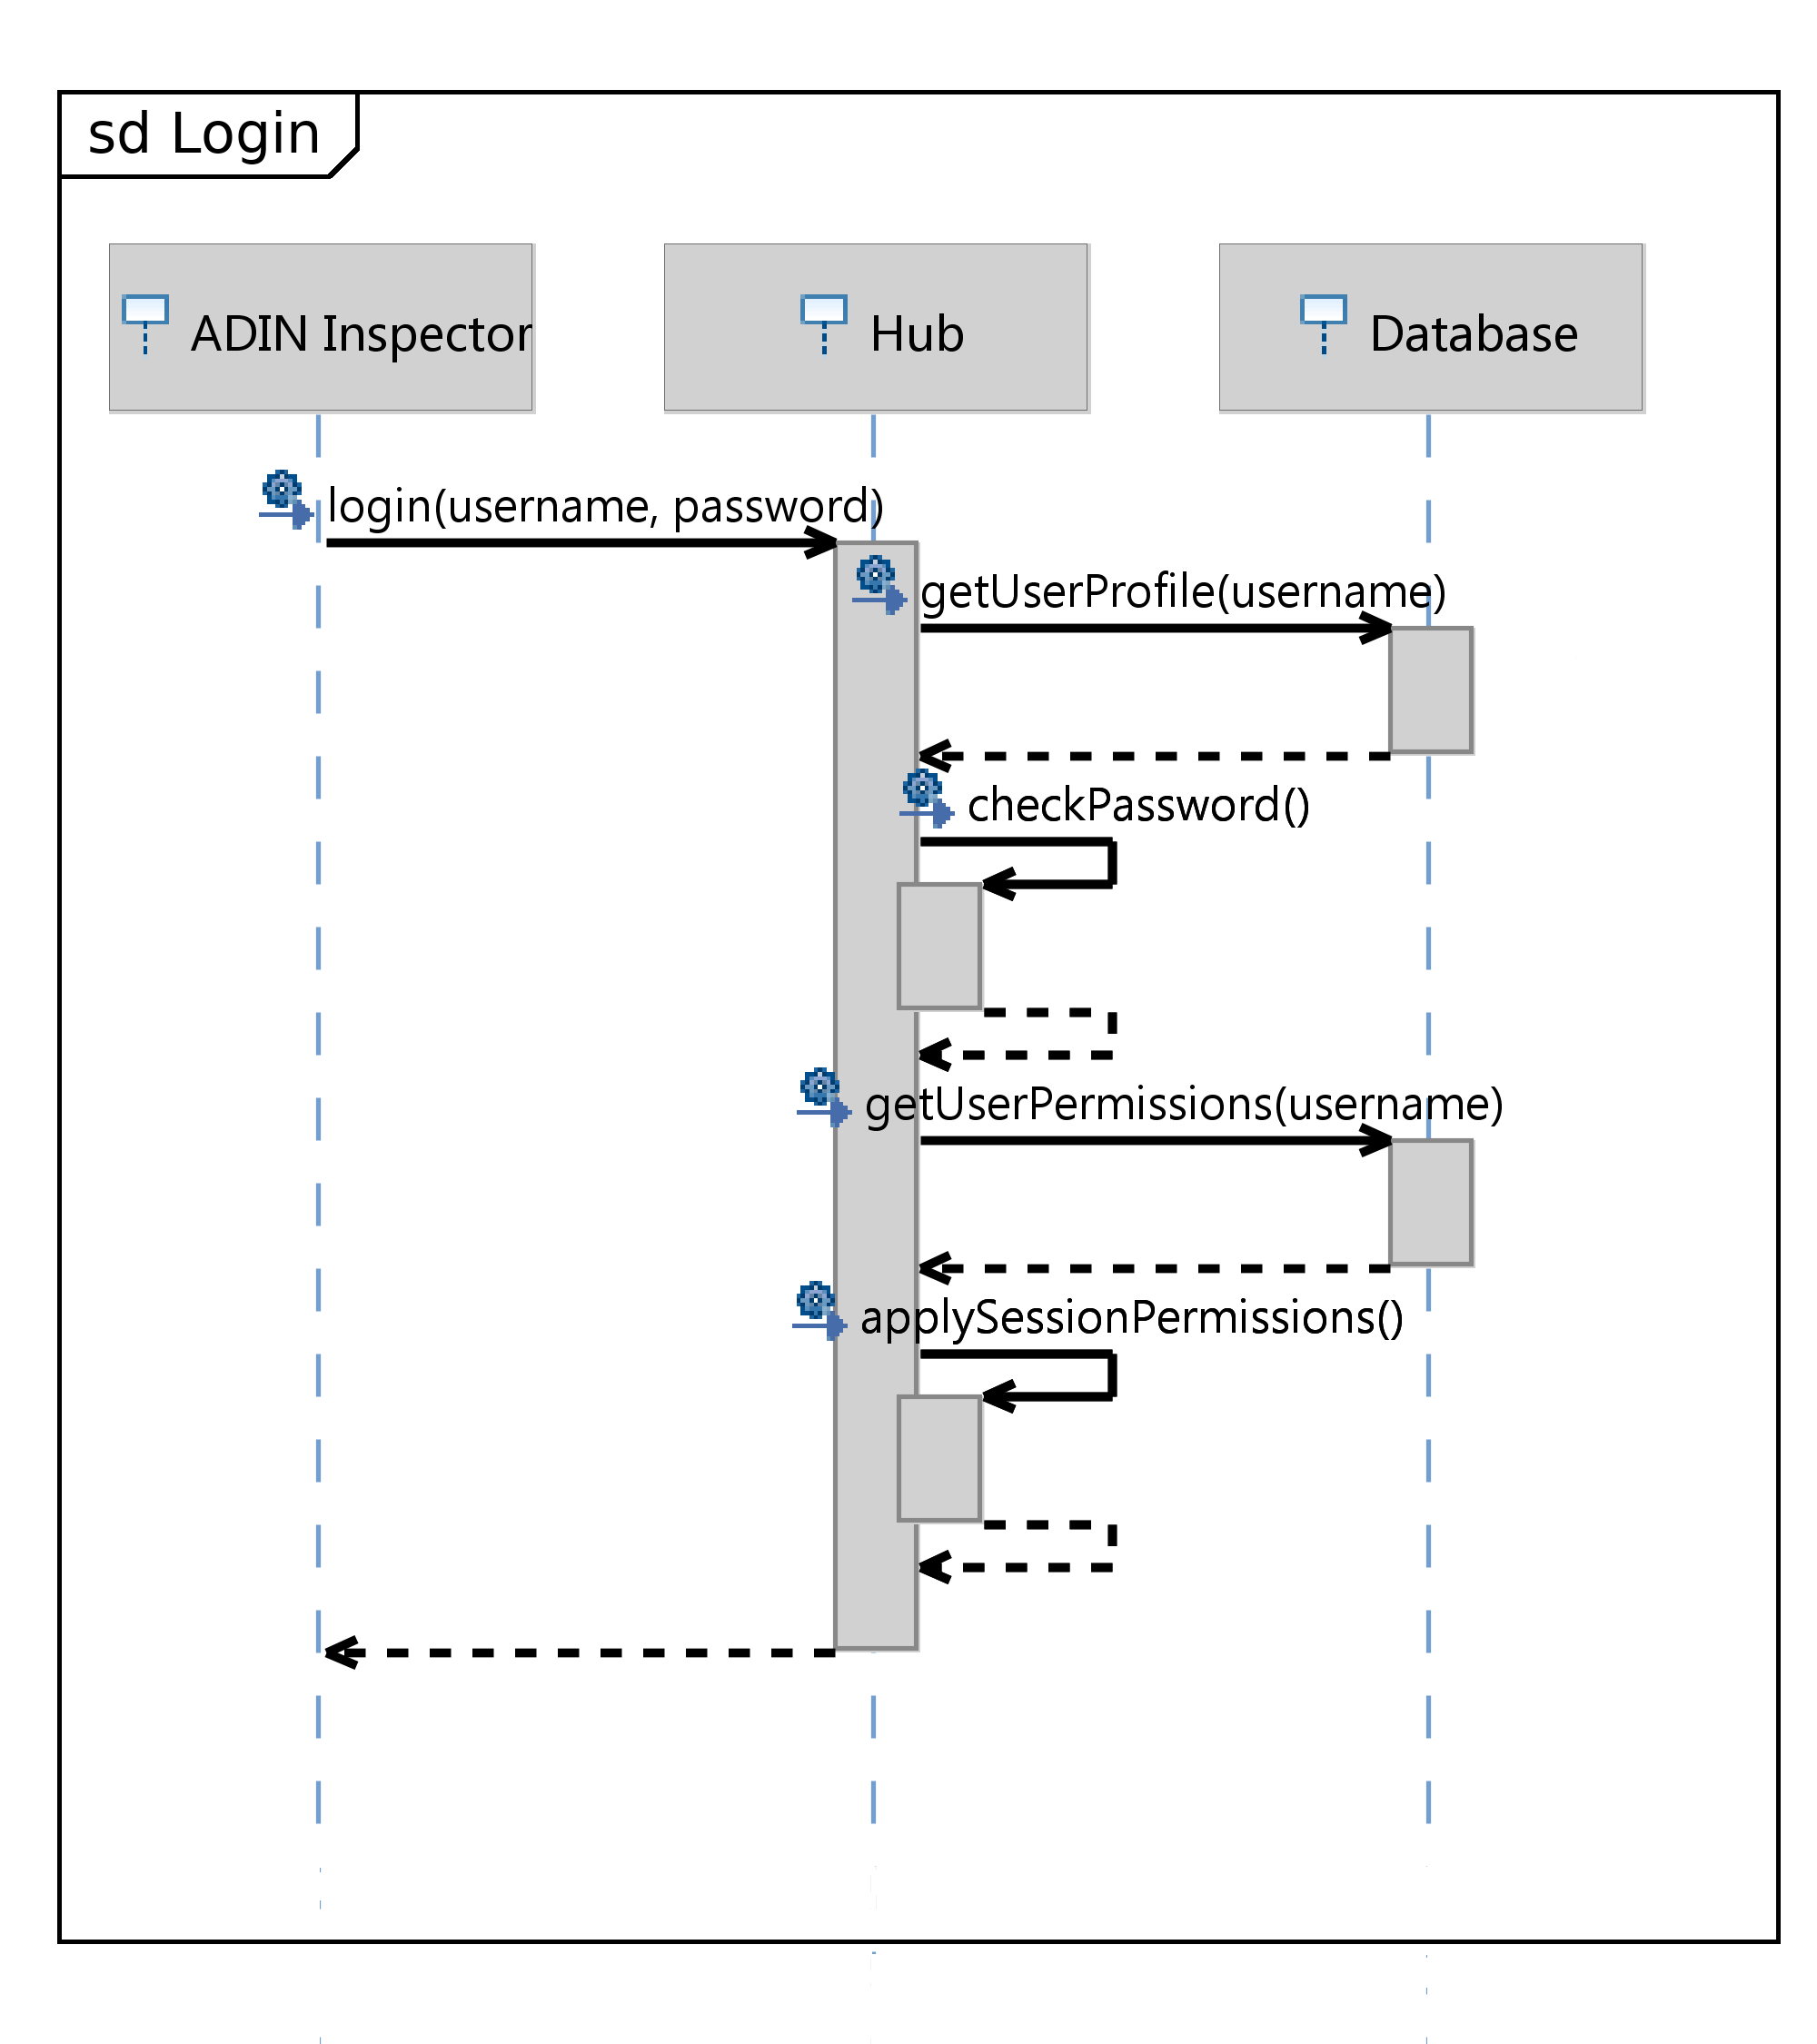
\includegraphics[width=0.8\textwidth]{Images/adin-login-seq.png}
\captionof{figure}{The activity of the Hub during login.}
\label{fig:adin-login-seq}
\end{center}

\section{Glossary}
\printglossary[title=,toctitle=]


%% |   Bibliography   |
%% --------------------

%% Add entry to the table of contents for the bibliography
\printbibliography[heading=bibintoc]

\end{document}
